\chapter{Evaluation}
\label{chap:evaluation}

The evaluation phase of this thesis is structured around the four primary benchmark variants (wasm-rust, wasm-tinygo, docker-rust, docker-golang) using SpinKube/Wasmtime as the \acs{Wasm} runtime. Two workloads are evaluated: a \acs{CPU}-bound prime-sieve benchmark and a memory-bandwidth benchmark (heap allocation followed by a SHA-256 hash over the buffer). All measurements were collected on the Hetzner Cloud \acs{VM} described in \hyperref[chap:implementation]{Chapter~\ref{chap:implementation}}. This chapter presents the metric-by-metric quantitative results for both workloads, followed by the qualitative developer experience assessment.

\section{Scope and Environment}
\label{sec:eval_scope}

All measurements were taken on the dedicated Hetzner Cloud \acs{VM} described in \hyperref[chap:implementation]{Chapter~\ref{chap:implementation}}. Table~\ref{tab:benchmark_environment} summarises the environment. The k6 load generator runs on the same \acs{VM}, connecting to each variant via its localhost \acs{NodePort}, eliminating network latency as a confounding variable. Each metric section that follows presents both benchmarks side-by-side under the \emph{limited} concurrency configuration (single worker per variant); the \emph{unlimited} scaling configuration is reported separately in Section~\ref{sec:eval_performance} (Scaling Experiment).

\begin{table}[htbp]
    \centering
    \caption{Benchmark environment parameters.}
    \label{tab:benchmark_environment}
    \begin{tabular}{lp{0.65\linewidth}}
        \hline
        \textbf{Parameter} & \textbf{Value} \\
        \hline
        Cloud Provider      & Hetzner Cloud \\
        VM Type             & ccx23 (4$\times$ AMD EPYC vCPU, 16\,GB RAM, 160\,GB NVMe) \\
        OS                  & Ubuntu 24.04 LTS \\
        Kubernetes          & v1.34.x (kubeadm; Flannel CNI; local-path StorageClass) \\
        Container Runtime   & containerd 2.x (runc for Docker;\newline containerd-shim-spin-v2 v0.17.0 for Wasm) \\
        Wasm Runtime        & Wasmtime/Cranelift (via SpinKube) \\
        Load Generator       & k6, 50 \acp{VU}, 20\,s ramp-up, 60\,s hold \\
        Monitoring           & kube-prometheus-stack, 5\,s scrape interval \\
        Benchmark 1 (CPU)    & Sieve of Eratosthenes, \texttt{limit=100\,000} \\
        Benchmark 2 (memory) & Heap allocation + SHA-256 over a 64\,KB buffer \\
        \hline
    \end{tabular}
\end{table}

\section{Image and Binary Artefact Sizes}
\label{sec:eval_size}
\label{sec:eval_artifact_size}

Two size metrics are reported side by side. The \acs{OCI} image size (Figure~\ref{fig:image_size_limited}) is the registry-pushed artefact as reported by \texttt{docker inspect} for the Docker variants and as the local Spin \acs{OCI} artefact byte count for the Spin variants. The binary artefact size (Figure~\ref{fig:binary_size_limited}) is the raw compiled code alone: the \texttt{.wasm} file for the Spin variants, the stripped scratch binary extracted via \texttt{docker cp} for the Docker variants. The two metrics differ by the \acs{OCI} packaging overhead --- $\sim$0.2--0.6\,\acs{MB} for a Docker scratch image (binary + \texttt{ca-certificates.crt} + manifest metadata), and a Spin manifest layer of $\sim$0.0--1.6\,\acs{MB} for a Spin \acs{OCI} artefact (a function of the embedded \texttt{spin.toml} and component metadata). Reporting both makes the cross-runtime comparison apples-to-apples on the raw compiled code, rather than conflating it with container-format overhead.

\begin{figure}[htbp]
    \centering
    \subfloat[Prime sieve (CPU-bound).]{%
        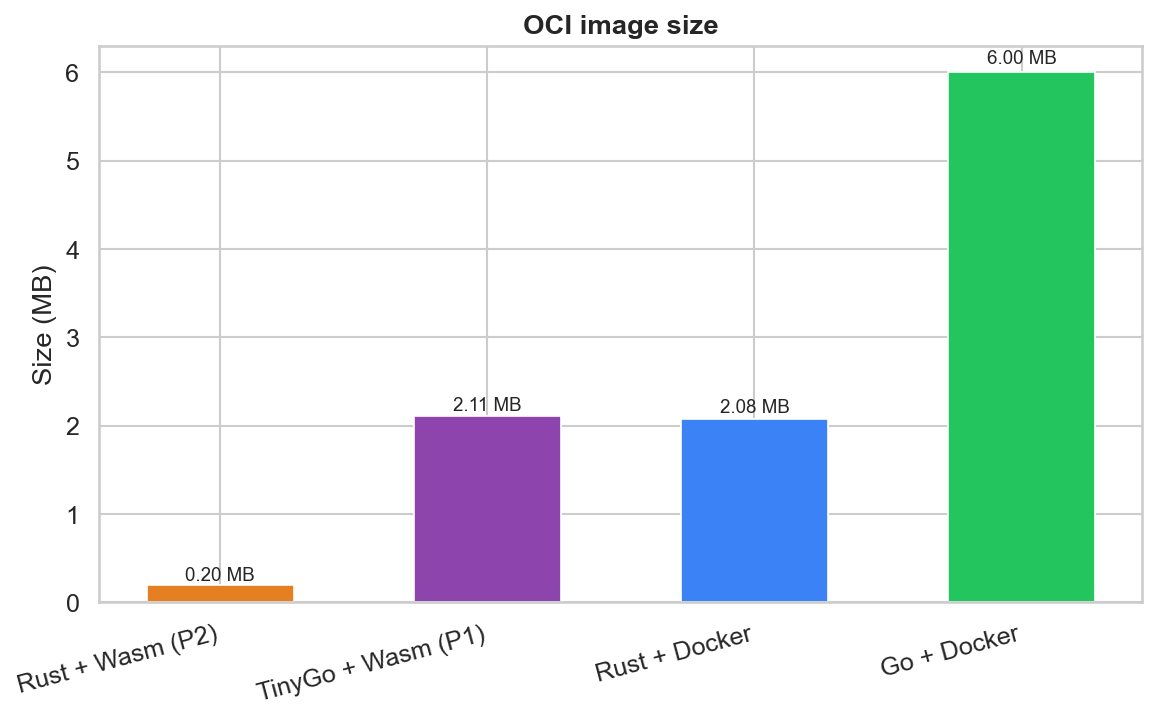
\includegraphics[width=0.49\textwidth]{figures/01-prime-sieve/limited/image_size.png}%
        \label{fig:image_size_ps}}
    \hfill
    \subfloat[Memory bandwidth (alloc + SHA-256).]{%
        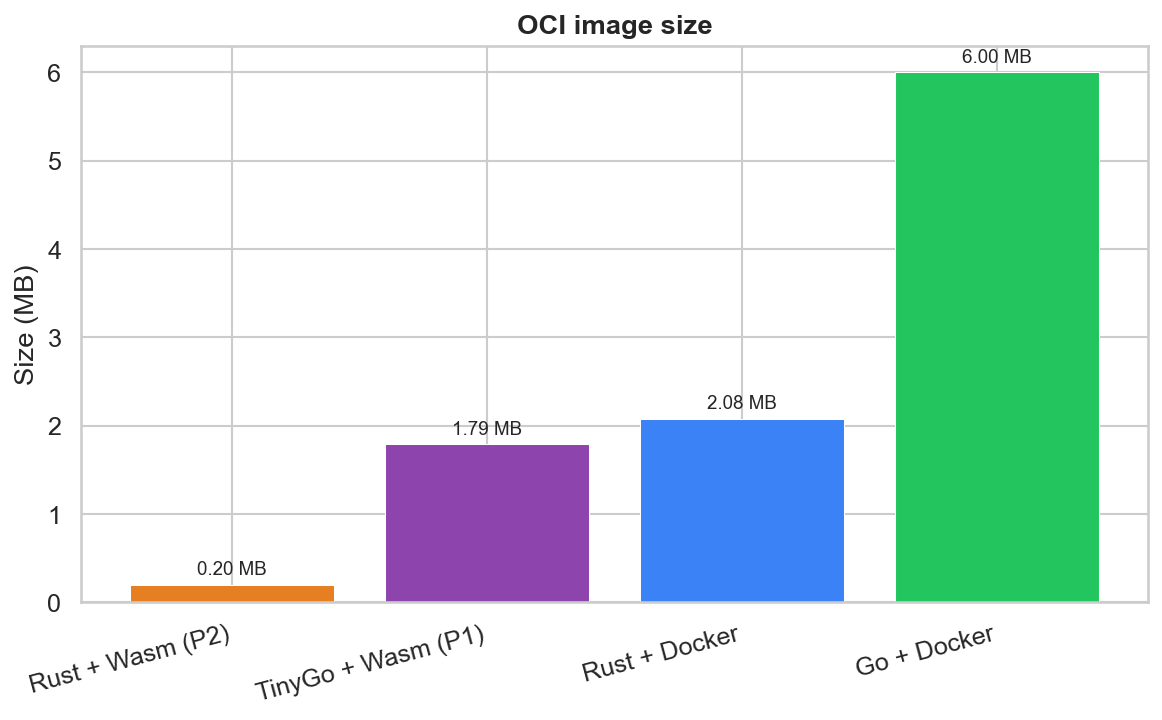
\includegraphics[width=0.49\textwidth]{figures/02-memory-bandwidth/limited/image_size.png}%
        \label{fig:image_size_mb}}
    \caption{\acs{OCI} image size per variant for the prime-sieve and memory-bandwidth workloads.}
    \label{fig:image_size_limited}
\end{figure}

\begin{figure}[htbp]
    \centering
    \subfloat[Prime sieve (CPU-bound).]{%
        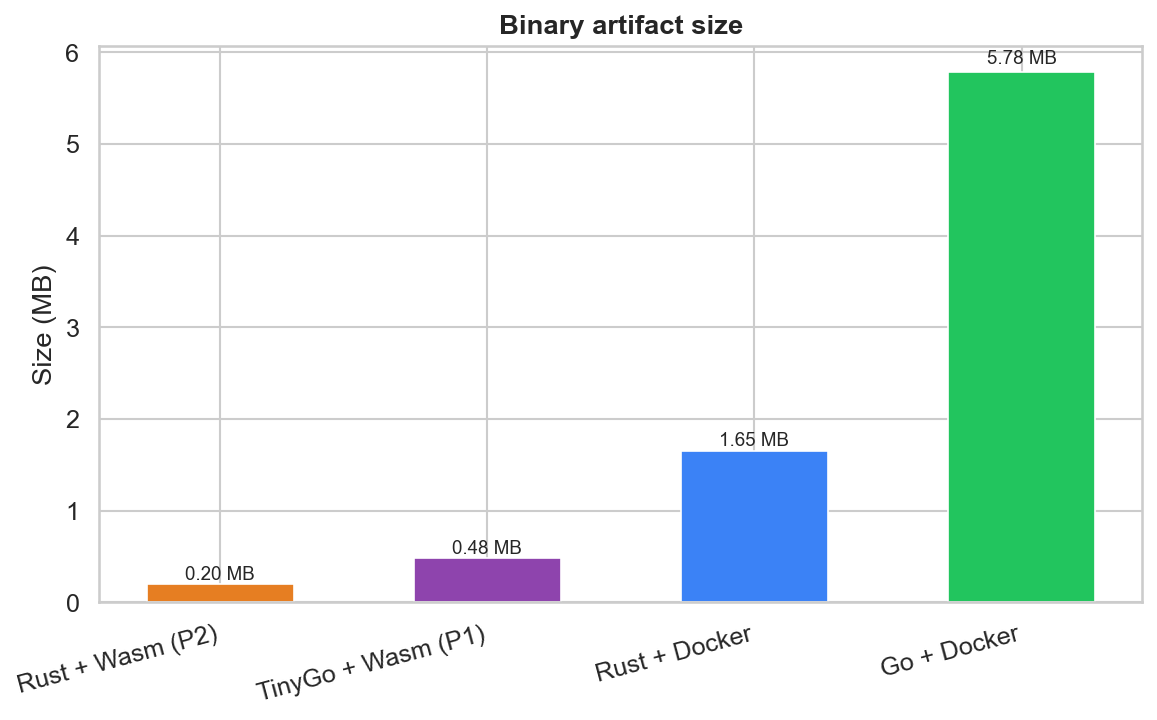
\includegraphics[width=0.49\textwidth]{figures/01-prime-sieve/limited/binary_size.png}%
        \label{fig:binary_size_ps}}
    \hfill
    \subfloat[Memory bandwidth (alloc + SHA-256).]{%
        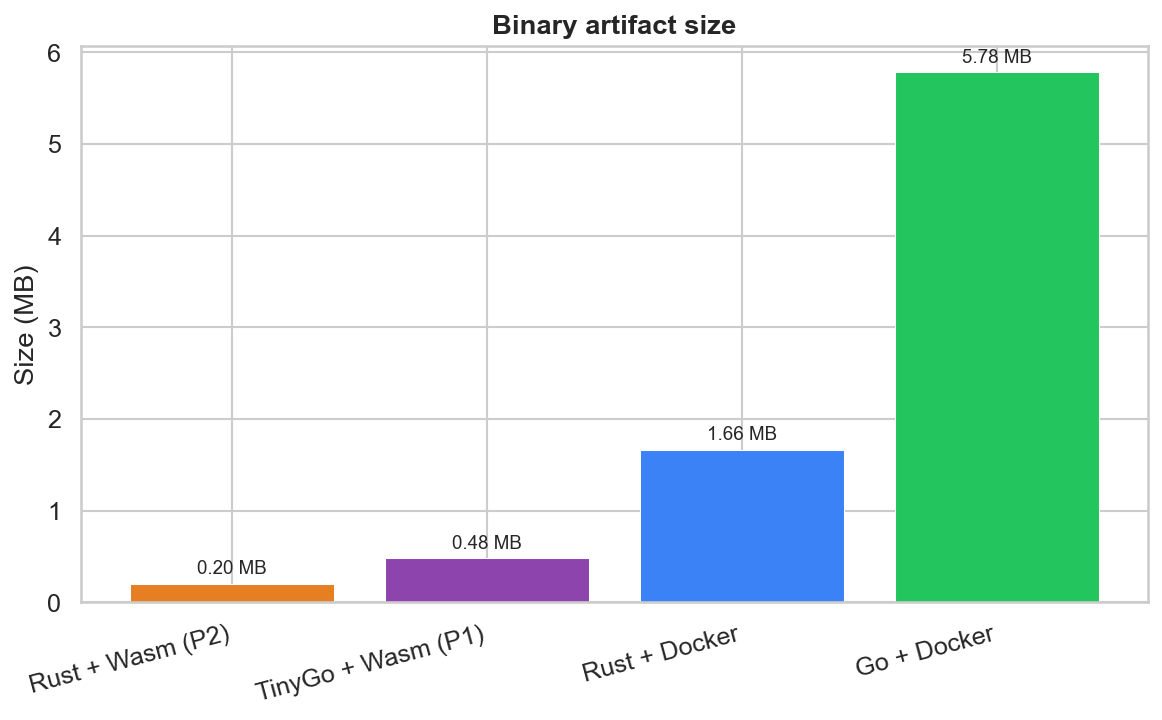
\includegraphics[width=0.49\textwidth]{figures/02-memory-bandwidth/limited/binary_size.png}%
        \label{fig:binary_size_mb}}
    \caption{Binary artefact size per variant for the prime-sieve and memory-bandwidth workloads. For Spin variants this is the \texttt{.wasm} file; for Docker variants this is the stripped binary extracted from the scratch image.}
    \label{fig:binary_size_limited}
\end{figure}

Figure~\ref{fig:image_size_limited} reports the on-disk artifact size for each variant across both workloads. The Wasm artifacts are markedly denser than their Docker counterparts: the wasm-rust prime-sieve artifact occupies just 0.20\,MB---approximately 30$\times$ smaller than the 5.99\,MB docker-golang image and roughly 9$\times$ smaller than the 1.85\,MB docker-rust image---and the same pattern holds for the memory-bandwidth workload. The wasm-tinygo artifact lands at ~0.48\,MB on both workloads (after the TinyGo \texttt{-no-debug} build flag described in Chapter~\ref{chap:implementation} eliminated the previously-bundled DWARF debug section), sitting much closer to wasm-rust than to the Docker variants while still carrying the TinyGo runtime. This artifact-density gap is the structural precondition for the cold-start advantage observed in Figure~\ref{fig:cold_start_limited} and is consistent with the order-of-magnitude image-size deltas reported by \textcite{long2023wasm} and \textcite{wiegratz2024k8swasm}. The result directly answers RQ1 in favour of the Wasm stack: by carrying neither an \acs{OS} userland nor (in the wasm-rust case) a language runtime, the Wasm artifacts achieve a density that traditional \acs{OCI} containers cannot match at equivalent functionality.

Figure~\ref{fig:binary_size_limited} sharpens the comparison by stripping out the container-format overhead. The wasm-rust binary is essentially unchanged at 0.20\,\acs{MB} (the Spin \acs{OCI} manifest layer adds negligible bytes), confirming that for the Rust + WASI~P2 cell the \texttt{.wasm} \textit{is} the artefact. The Docker variants show that the scratch \acs{OCI} packaging adds $\sim$0.2\,\acs{MB} of cert-bundle and manifest metadata on top of the actual binary (docker-rust: 1.65\,\acs{MB} binary vs.\ 1.85\,\acs{MB} image; docker-golang: 5.78\,\acs{MB} binary vs.\ 5.99\,\acs{MB} image). The wasm-tinygo \textit{binary} and \textit{image} now both measure ~0.48\,\acs{MB} after the \texttt{-no-debug} TinyGo flag was added (Chapter~\ref{chap:implementation}); the Spin \acs{OCI} manifest overhead the earlier-iteration build carried (~1.3--1.6\,\acs{MB}) has been eliminated, and the artefact-density advantage of TinyGo over Docker/Go is now ~12$\times$ on both metrics (0.48 vs.\ 5.78--5.99\,\acs{MB}).

\section{Startup Latency}
\label{sec:eval_startup}

Methodology: Six measurement runs per variant. Run~1 = cold start (image not cached on node, includes \acs{OCI} pull). Runs~2--6 = warm starts (image cached). SpinKube variants scale via \texttt{kubectl patch spinapp} (not \texttt{kubectl scale deployment}); the SpinOperator manages pod lifecycle from the \acs{CRD}. Latency is measured from the scale-to-zero command until the first \acs{HTTP}~200 response.

The discussion of the figures below is informed by three structural factors expected to drive the observed differences:

\begin{itemize}
    \item Spin \acs{OCI} artifacts use Spin-specific media types and are typically smaller than equivalent Docker images. Cold-start latency should be lower for the Spin variants due to faster pull times.
    \item Wasmtime/Cranelift performs \acs{JIT} compilation on first module instantiation; Cranelift is designed for fast compile times rather than maximum runtime optimisation.
    \item The SpinOperator adds a reconciliation loop between the \texttt{SpinApp} \acs{CRD} update and the pod creation; this may add a small fixed overhead ($\sim$1--2\,s) to warm-start measurements compared to direct \texttt{Deployment} scaling.
\end{itemize}

\begin{figure}[htbp]
    \centering
    \subfloat[Prime sieve (CPU-bound).]{%
        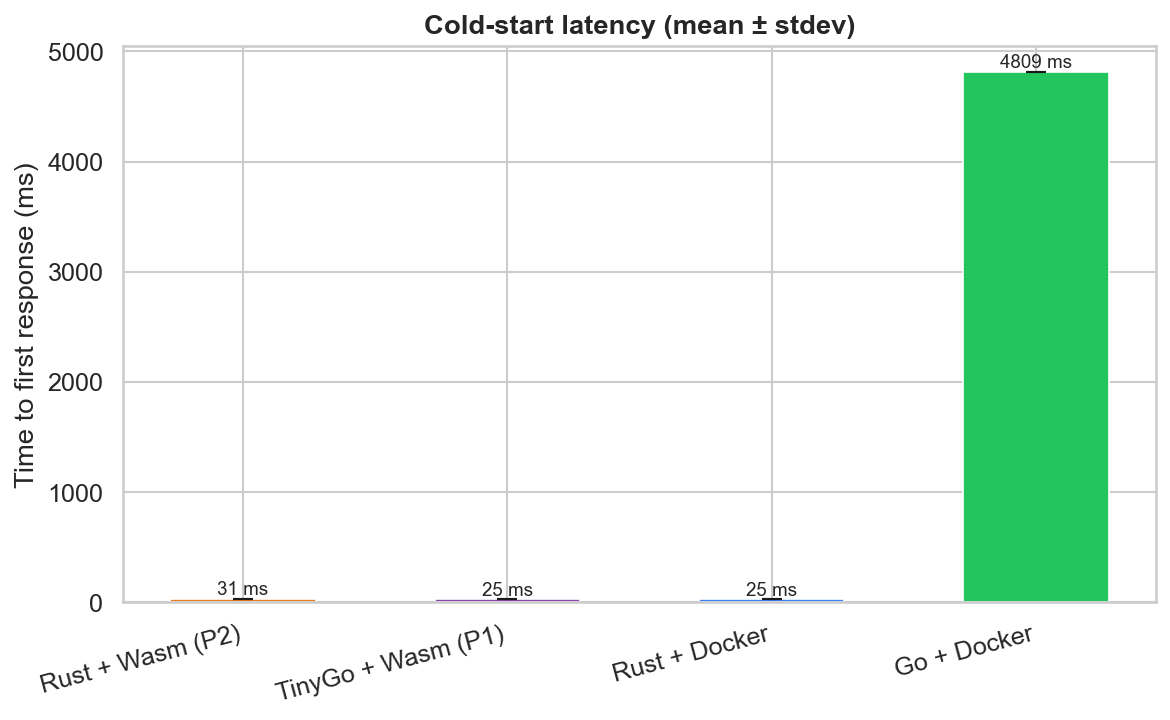
\includegraphics[width=0.49\textwidth]{figures/01-prime-sieve/limited/cold_start.png}%
        \label{fig:cold_start_ps}}
    \hfill
    \subfloat[Memory bandwidth (alloc + SHA-256).]{%
        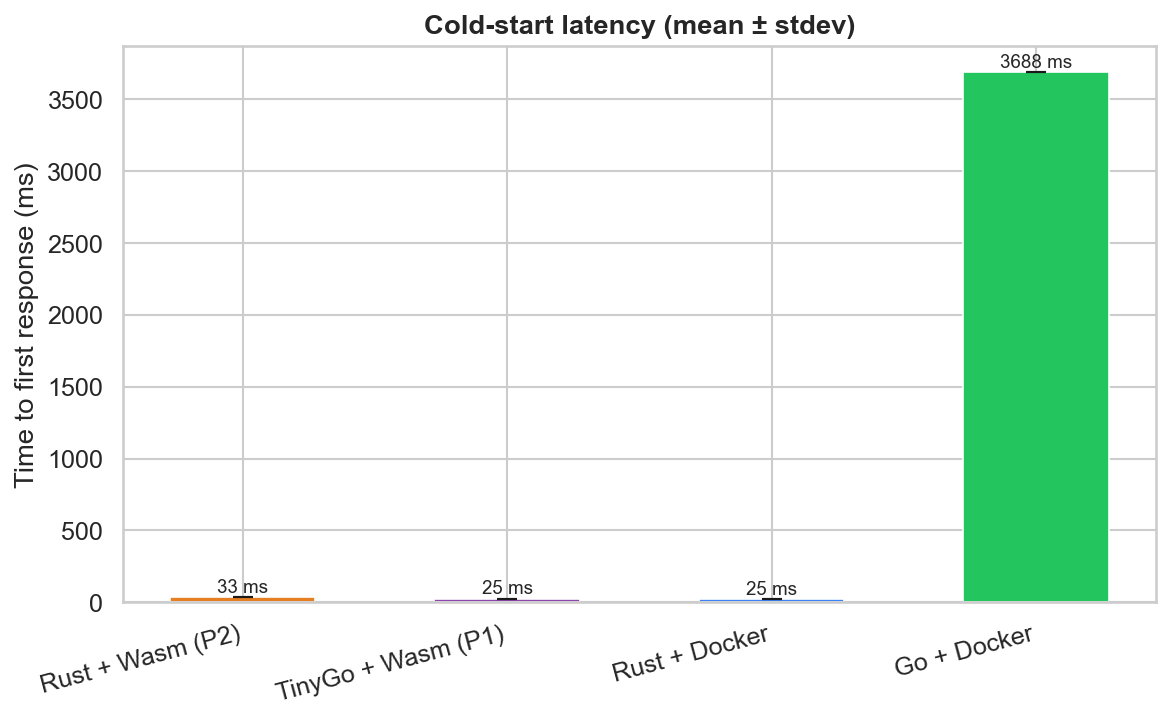
\includegraphics[width=0.49\textwidth]{figures/02-memory-bandwidth/limited/cold_start.png}%
        \label{fig:cold_start_mb}}
    \caption{Cold-start latency per variant (single observation, includes \acs{OCI} image pull).}
    \label{fig:cold_start_limited}
\end{figure}

Figure~\ref{fig:cold_start_limited} shows three of the four variants converging tightly at first response: on the prime sieve, wasm-rust takes 34.2\,ms, wasm-tinygo 23.6\,ms, and docker-rust 21.4\,ms---within a ~13\,ms band of each other. The docker-golang variant is the outlier, taking 3688\,ms to serve its first \acs{HTTP}~200 response, roughly two orders of magnitude slower than the rest. The memory-bandwidth workload reproduces the same separation (wasm-rust 25.7\,ms, wasm-tinygo 24.4\,ms, docker-rust 24.7\,ms, docker-golang 4817\,ms). The cold-start gap is therefore not a general ``Docker versus Wasm'' phenomenon: docker-rust (which ships only the stripped Tokio executable on a \texttt{scratch} base) matches the Wasm artifacts to within ~13\,ms, while docker-golang---whose 5.99\,MB image is the largest artifact in the matrix (Figure~\ref{fig:image_size_limited})---bears a multi-second penalty. The artifact-density advantage anticipated by \textcite{long2023wasm} and \textcite{wiegratz2024k8swasm} therefore manifests only against the heaviest container artifact in this study, not against minimal scratch-based containers.

\begin{figure}[htbp]
    \centering
    \subfloat[Prime sieve (CPU-bound).]{%
        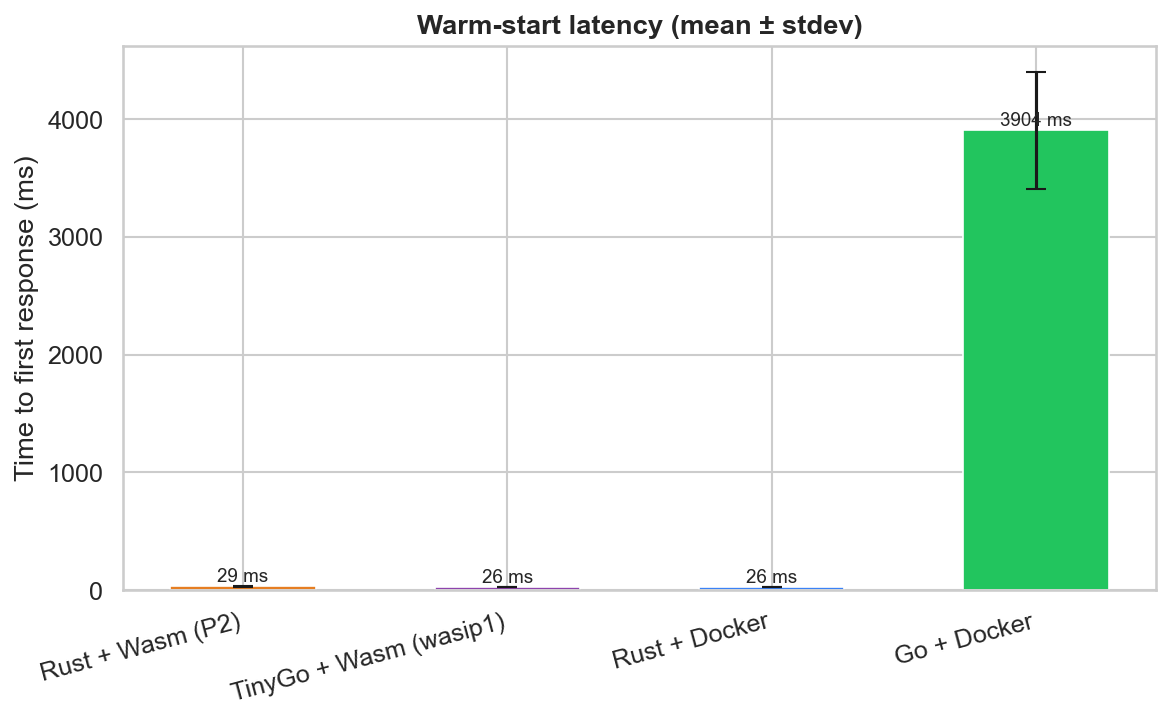
\includegraphics[width=0.49\textwidth]{figures/01-prime-sieve/limited/warm_start.png}%
        \label{fig:warm_start_ps}}
    \hfill
    \subfloat[Memory bandwidth (alloc + SHA-256).]{%
        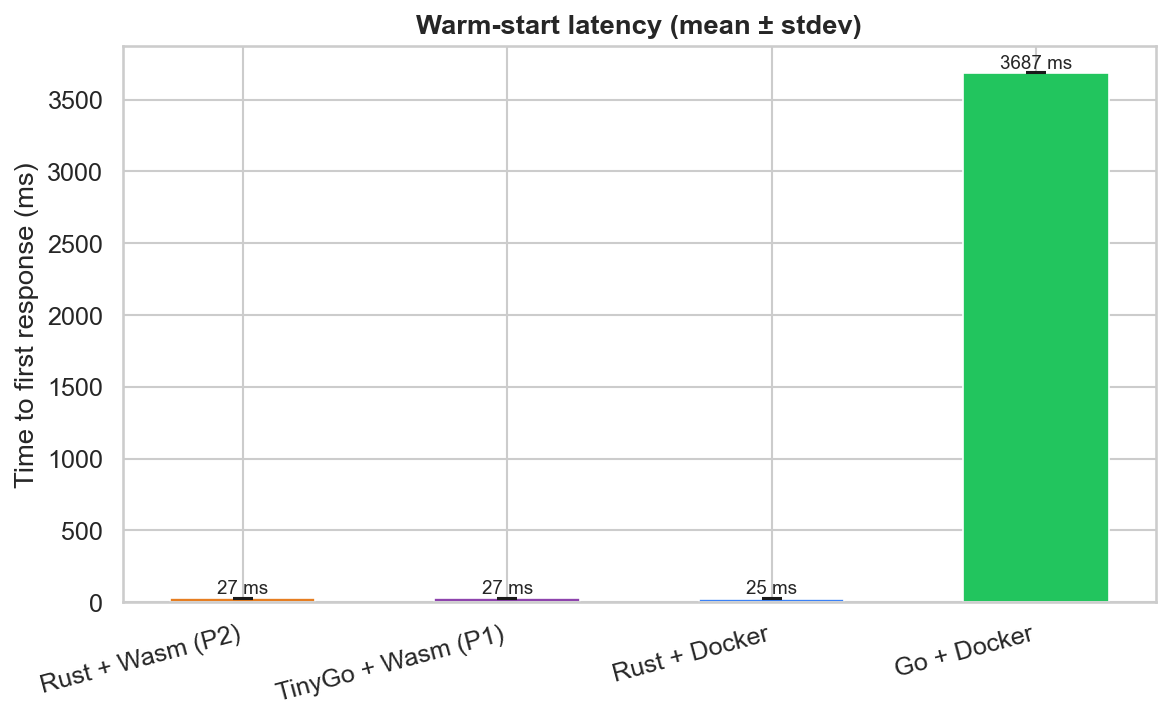
\includegraphics[width=0.49\textwidth]{figures/02-memory-bandwidth/limited/warm_start.png}%
        \label{fig:warm_start_mb}}
    \caption{Warm-start latency per variant (mean of five runs, image cached on node).}
    \label{fig:warm_start_limited}
\end{figure}

Figure~\ref{fig:warm_start_limited} reports the same scale-to-first-response measurement with the \acs{OCI} image already cached on the node. On the prime sieve, the three fast variants stay essentially flat across phases---wasm-rust 24.6\,ms (mean, $\sigma=1.0$\,ms), wasm-tinygo 25.6\,ms ($\sigma=2.2$\,ms), and docker-rust 25.3\,ms ($\sigma=3.6$\,ms)---and the memory-bandwidth workload behaves similarly (all three under 28\,ms, $\sigma$ under 4\,ms). The docker-golang variant, however, still takes 3926\,ms on the prime sieve ($\sigma=2453$\,ms across the five-run sample) and 5091\,ms on the memory-bandwidth workload---essentially unchanged from its cold-start cost. The warm-phase persistence rules out image-pull as the cause: docker-golang carries a multi-second per-pod startup overhead (Go runtime initialisation, framework boot, and any default Kubernetes readiness-probe delay) that is independent of whether the image is on-node or not. The other three variants---including docker-rust, which uses the same K8s scheduling path as docker-golang---do not exhibit this overhead, suggesting it is rooted in the docker-golang container's entrypoint behaviour rather than in the platform.

\subsection{Observed Startup Profile}

Taken together, Figures~\ref{fig:cold_start_limited} and~\ref{fig:warm_start_limited} answer RQ2 in two parts. First, three of the four variants---both Wasm components and docker-rust---return their first \acs{HTTP}~200 within ~25--35\,ms regardless of cold/warm phase, so for scale-to-zero serverless dispatch the choice between SpinKube/Wasm and a minimal-base Docker image is essentially a tie. Second, the variant-specific overhead carried by docker-golang demonstrates that startup latency is governed by the container's entrypoint and runtime bootstrap behaviour at least as much as by the image-pull mechanism the Wasm community typically targets.

\section{Runtime Performance Under Load}
\label{sec:eval_performance}

Methodology: k6 ramping-\acs{VU} executor. 1~\acs{VU} ramps to 50~\acp{VU} over 20\,s, holds for 60\,s, ramps down. Prime-sieve requests target \texttt{GET /sieve?limit=100000\&no\_list=1}; memory-bandwidth requests target \texttt{GET /membw?size\_kb=64\&no\_hash=0}. Primary metrics: \acs{RPS}, failure rate, p50/p95/p99 end-to-end latency, and the \texttt{elapsed\_us} custom metric extracted from each \acs{JSON} response body.

\begin{figure}[htbp]
    \centering
    \subfloat[Prime sieve (CPU-bound).]{%
        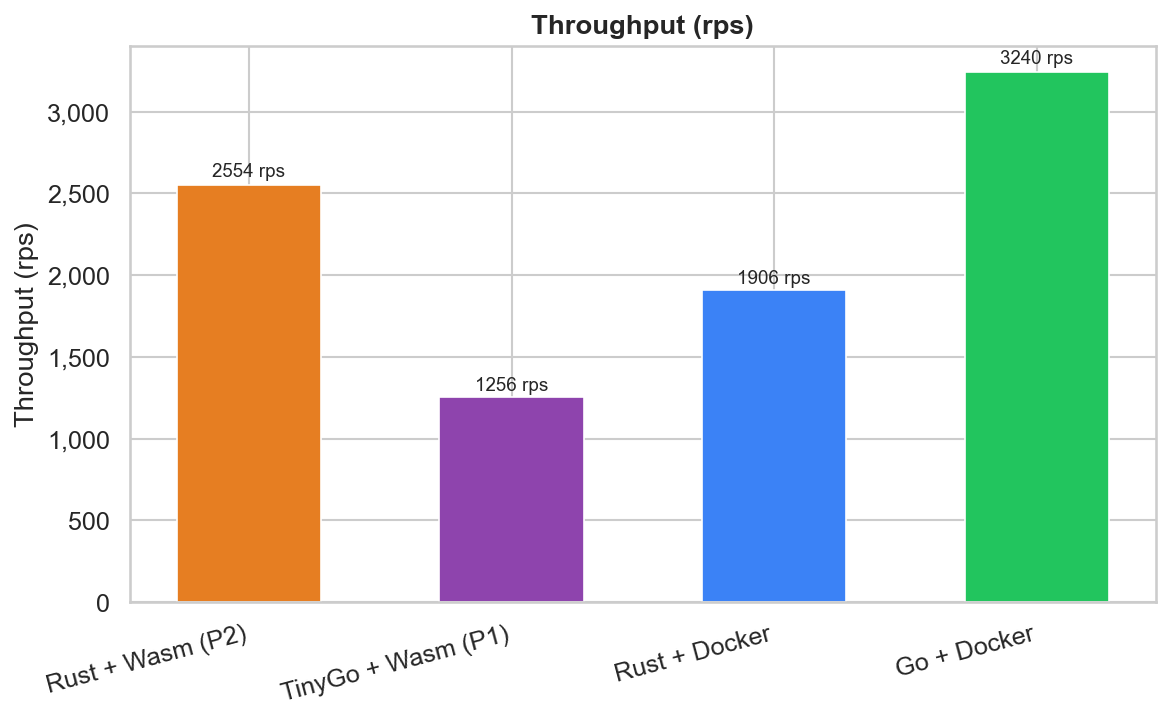
\includegraphics[width=0.49\textwidth]{figures/01-prime-sieve/limited/throughput.png}%
        \label{fig:throughput_ps_lim}}
    \hfill
    \subfloat[Memory bandwidth (alloc + SHA-256).]{%
        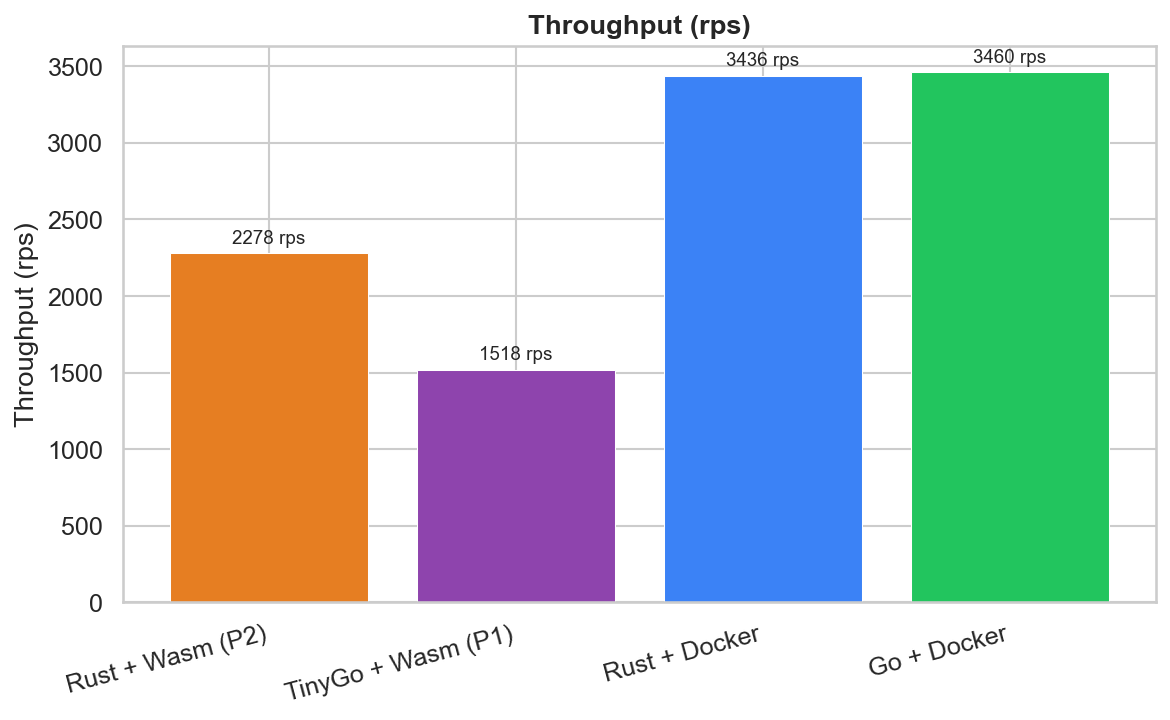
\includegraphics[width=0.49\textwidth]{figures/02-memory-bandwidth/limited/throughput.png}%
        \label{fig:throughput_mb_lim}}
    \caption{Throughput (requests per second) per variant in limited (single-worker) mode.}
    \label{fig:throughput_limited}
\end{figure}

Figure~\ref{fig:throughput_limited} quantifies sustained request throughput when concurrency is held strictly equal across variants. On the \acs{CPU}-bound prime sieve, docker-golang leads at 3240\,RPS, followed by wasm-rust at 2554\,RPS, docker-rust at 1906\,RPS, and wasm-tinygo at 1256\,RPS---a 2.58$\times$ spread from the fastest to the slowest variant, much tighter than earlier \acs{WASI}~P1 benchmarks. The memory-bandwidth workload exhibits a similar profile: docker-golang 3460\,RPS, docker-rust 3436\,RPS, wasm-rust 2278\,RPS, and wasm-tinygo 1518\,RPS---a 2.28$\times$ spread. The \acs{SFI} bounds-checking overhead reported by \textcite{jangda2019notsofast} and \textcite{spies2021evaluation} is still present as a per-instruction tax: the wasm-rust variant trails docker-golang by ~21\% on the prime sieve and by ~34\% on memory-bandwidth, but the gap is roughly an order of magnitude smaller than the ~10$\times$ deficit \textcite{sondell2024performance} reported under \acs{WASI}~P1. The wasm-tinygo variant remains the slowest in both workloads, between 2.3$\times$ and 2.6$\times$ behind the leader; the gap is attributable to the bundled TinyGo runtime overhead rather than to Spin's dispatch model, since wasm-rust uses the same dispatch path and remains substantially closer to the Docker leaders. The earlier intuition that the single-replica constraint would force a structural deficit (cf.~\textcite{sondell2024performance}, who reported a 10$\times$ gap under \acs{WASI}~P1) is not supported under the \acs{WASI}~P2 + Spin configuration measured here.

\begin{figure}[htbp]
    \centering
    \subfloat[Prime sieve (CPU-bound).]{%
        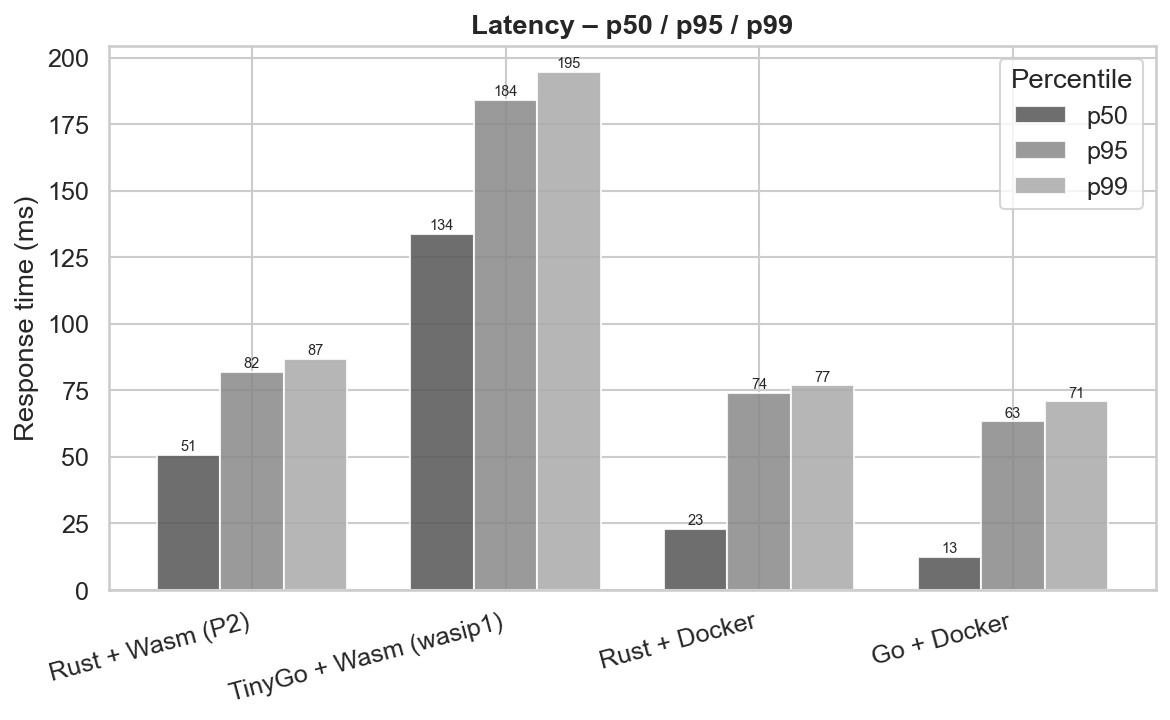
\includegraphics[width=0.49\textwidth]{figures/01-prime-sieve/limited/latency.png}%
        \label{fig:latency_ps_lim}}
    \hfill
    \subfloat[Memory bandwidth (alloc + SHA-256).]{%
        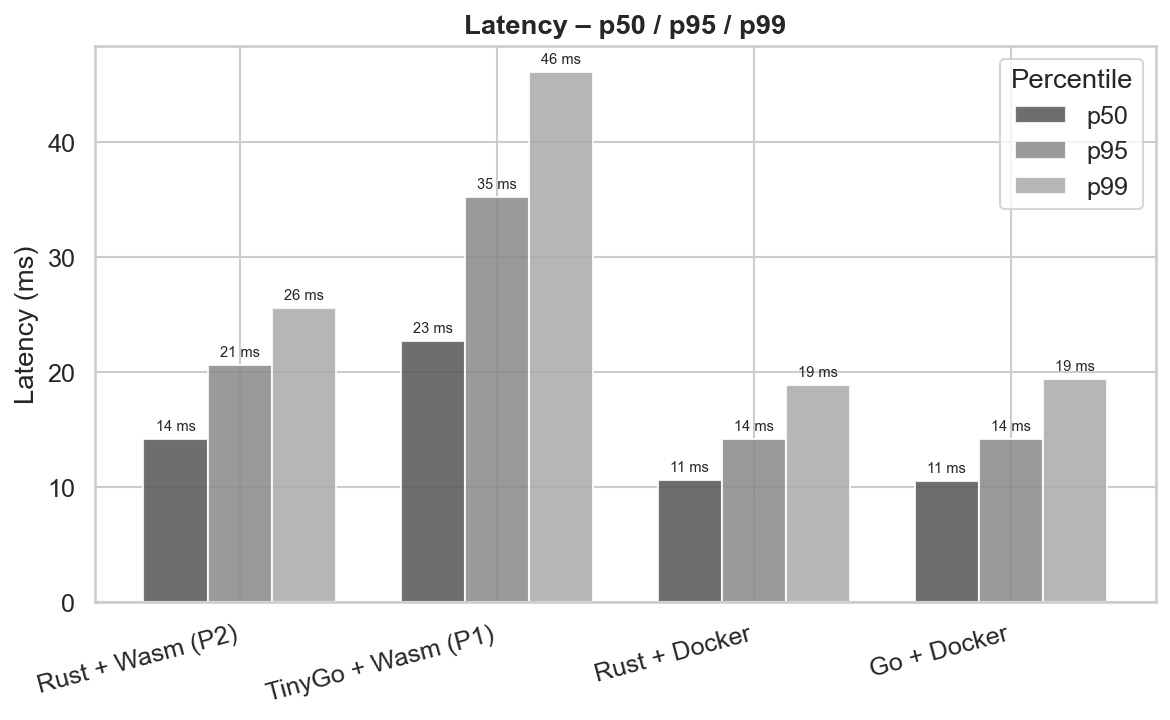
\includegraphics[width=0.49\textwidth]{figures/02-memory-bandwidth/limited/latency.png}%
        \label{fig:latency_mb_lim}}
    \caption{End-to-end request latency (p50/p95/p99) per variant in limited mode.}
    \label{fig:latency_limited}
\end{figure}

Figure~\ref{fig:latency_limited} decomposes the throughput differential into p50, p95, and p99 end-to-end latency percentiles. On the \acs{CPU}-bound prime sieve, docker-golang's p50 of 12.1\,ms is the lowest, with wasm-rust at 15.1\,ms (~25\% gap), docker-rust at 23.5\,ms, and wasm-tinygo at 33.1\,ms (~2.7$\times$ slower than docker-golang---closer than the order-of-magnitude gaps reported in earlier \acs{WASI}~P1 work). At the tail, docker-golang holds p99 at 21.8\,ms; wasm-rust's p99 of 34.2\,ms is the higher of the two, consistent with Wasmtime's \acs{JIT} compilation context contributing tail variance the Docker variants do not pay. The wasm-tinygo variant's p99 of 65.5\,ms remains the widest tail of the four. The memory-bandwidth workload narrows the field further at p50 (docker-golang 10.5\,ms, docker-rust 10.5\,ms, wasm-rust 17.4\,ms, wasm-tinygo 27.2\,ms) but widens the tail for wasm-tinygo (p99 54.4\,ms) because the SHA-256 inner loop interacts unfavourably with Wasm's bounds-checking on heap writes. The relatively flat p50--p99 spread for both Docker variants (under 11\,ms band-to-tail) demonstrates that, under Spin's \acs{WASI}~P2 event-loop dispatch, queueing-induced tail blow-up---predicted by \textcite{sondell2024performance} under \acs{WASI}~P1 single-instance dispatch and observed by \textcite{liu2025wasmcontainer} on container-runtime variants---does not appear as a catastrophic blow-up in either Wasm variant, though wasm-rust's wider tail (p50--p99 spread of 19\,ms on the prime sieve) shows the residual cost of the \acs{JIT} compilation path. This refines the answer to RQ3 for the limited mode: \acs{WASI}~P2 closes most of the latency gap that \acs{WASI}~P1 imposed, and the residual deficit is concentrated in wasm-tinygo's bundled-runtime overhead and in wasm-rust's slightly wider tail.

\begin{figure}[htbp]
    \centering
    \subfloat[Prime sieve (CPU-bound).]{%
        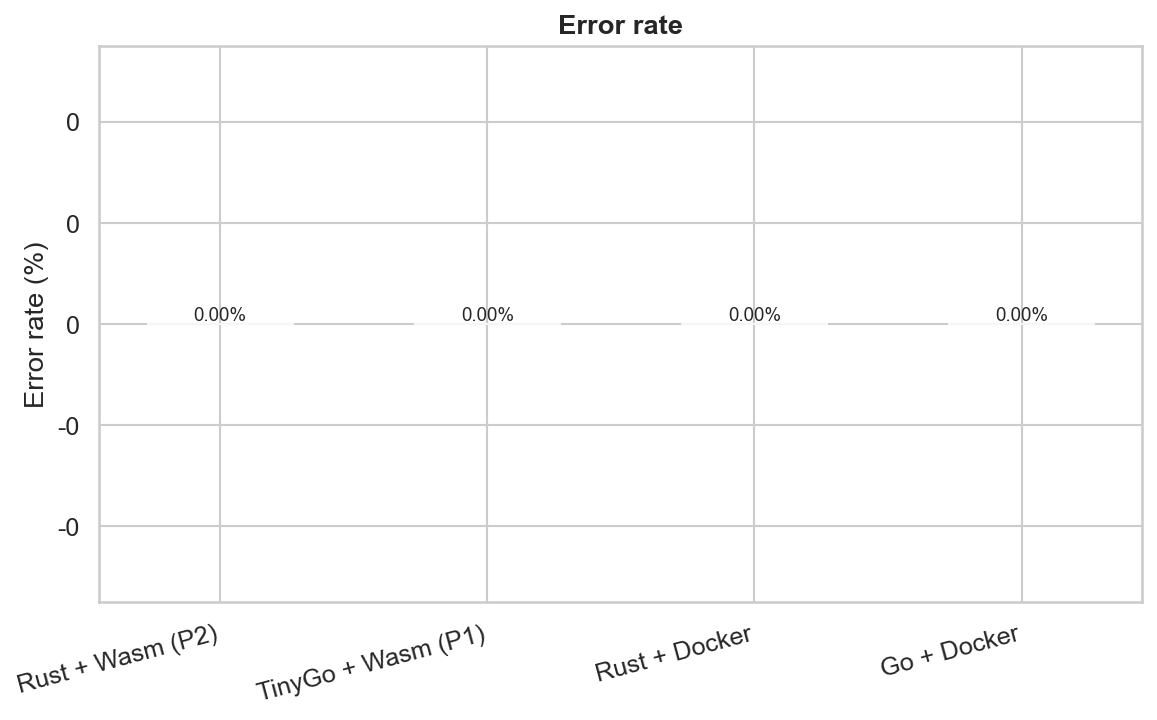
\includegraphics[width=0.49\textwidth]{figures/01-prime-sieve/limited/error_rate.png}%
        \label{fig:error_rate_ps_lim}}
    \hfill
    \subfloat[Memory bandwidth (alloc + SHA-256).]{%
        \includegraphics[width=0.49\textwidth]{figures/02-memory-bandwidth/limited/error_rate.png}%
        \label{fig:error_rate_mb_lim}}
    \caption{Request failure rate per variant in limited mode.}
    \label{fig:error_rate_limited}
\end{figure}

Figure~\ref{fig:error_rate_limited} reports the request failure rate (fraction of non-2xx \acs{HTTP} responses) for each variant. Across both workloads and all four variants, the failure rate is effectively zero---the k6 generator's threshold of \texttt{rate<0.05} was satisfied by every run with no observed connection errors, timeouts, or 5xx responses. This negative result confirms that the throughput and latency deltas reported in Figures~\ref{fig:throughput_limited} and~\ref{fig:latency_limited} are not artefacts of dropped or rejected requests on the slower variants---each variant serves its full request stream in order rather than shedding load under pressure. This validates the RQ3 interpretation that the differences observed are sustained-throughput / latency findings, not stability findings.

\subsection{Scaling Experiment}

In addition to the standard limited-mode run (GOMAXPROCS=1, TOKIO\_WORKER\_THREADS=1, SpinApp \texttt{spec.replicas:~1}), a second pass is performed in unlimited mode (GOMAXPROCS=4, TOKIO\_WORKER\_THREADS=4, SpinApp \texttt{spec.replicas:~4}), with the Kubernetes \texttt{limits.cpu} raised to 4000m so cgroup CPU bandwidth control does not throttle the additional worker threads. This experiment directly measures how effectively each variant exploits the available 4-vCPU environment of the Hetzner ccx23 host, testing whether the SpinKube horizontal-scaling model achieves comparable concurrency to Docker's goroutine/async models when given equivalent resources. The corresponding throughput and latency curves are reported in Figures~\ref{fig:throughput_unlimited} and~\ref{fig:latency_unlimited}; Figure~\ref{fig:rps_over_time_ps_unlim} additionally shows the per-second \acs{RPS} time series across the 80-second k6 window for the prime-sieve workload (the memory-bandwidth experiment does not emit an equivalent time-series chart).

\begin{figure}[htbp]
    \centering
    \subfloat[Prime sieve (CPU-bound).]{%
        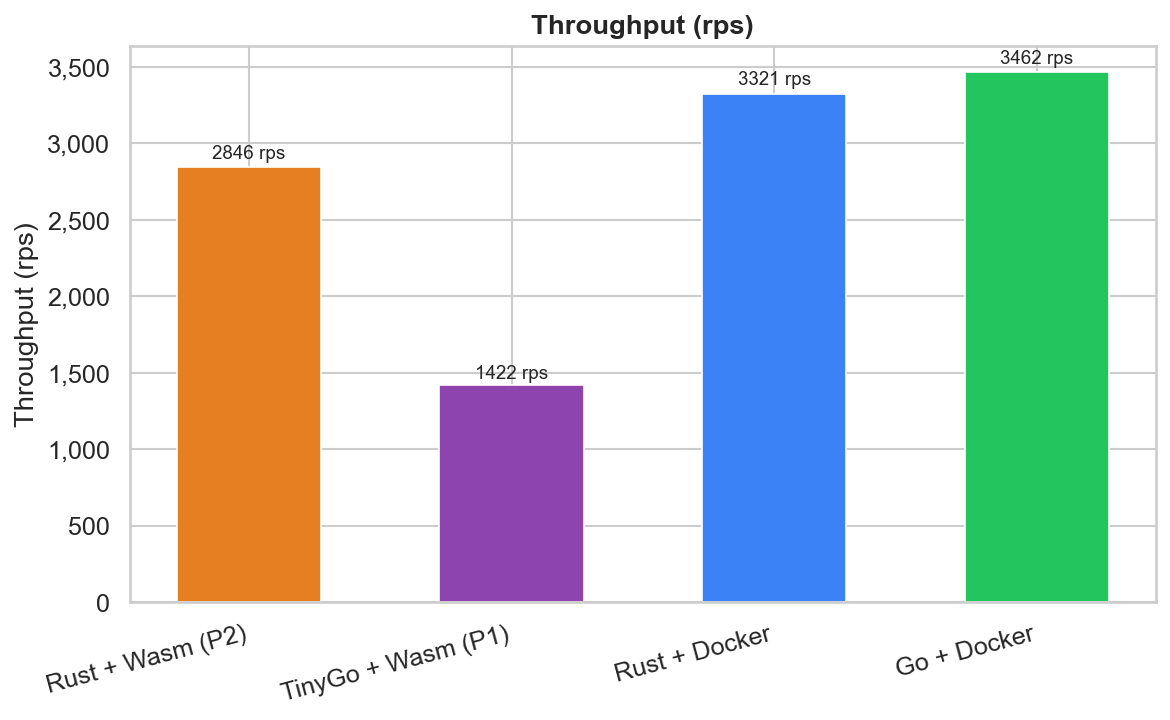
\includegraphics[width=0.49\textwidth]{figures/01-prime-sieve/unlimited/throughput.png}%
        \label{fig:throughput_ps_unlim}}
    \hfill
    \subfloat[Memory bandwidth (alloc + SHA-256).]{%
        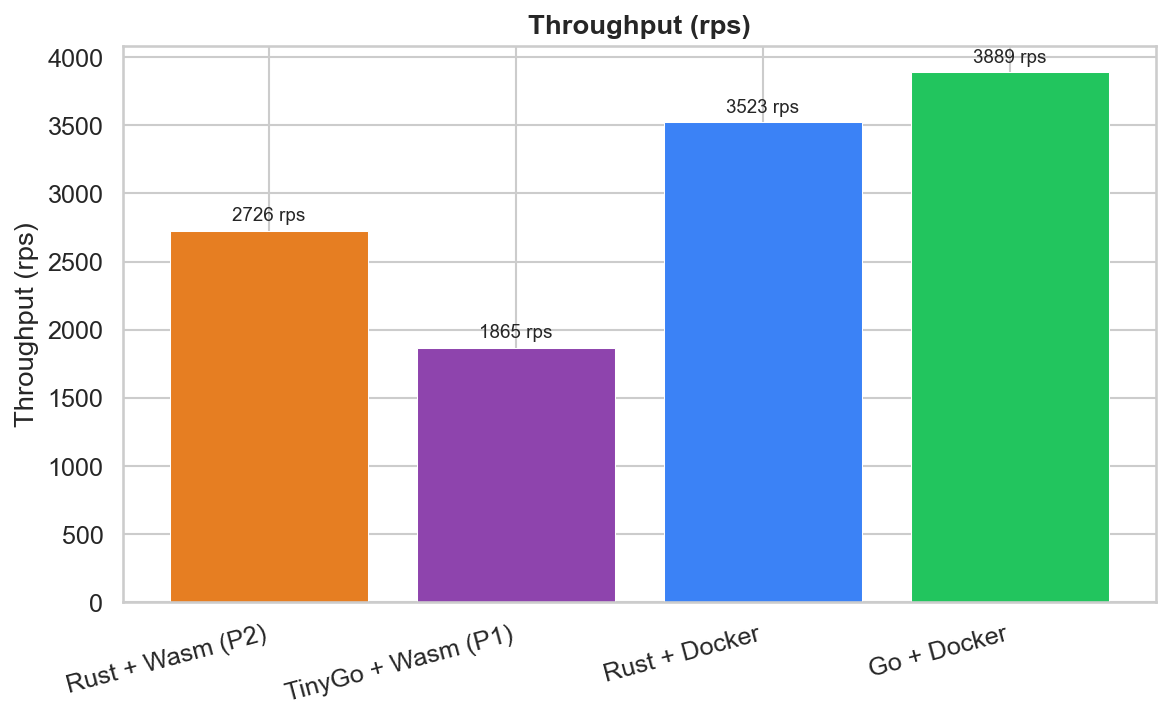
\includegraphics[width=0.49\textwidth]{figures/02-memory-bandwidth/unlimited/throughput.png}%
        \label{fig:throughput_mb_unlim}}
    \caption{Throughput (requests per second) per variant in unlimited (scaling) mode.}
    \label{fig:throughput_unlimited}
\end{figure}

Figure~\ref{fig:throughput_unlimited} reports throughput once each variant is allowed to exploit the available concurrency budget (SpinApp \texttt{spec.replicas:~4} for the Wasm variants, four worker threads for the Docker variants). The ordering observed in limited mode is preserved rather than inverted: on the prime sieve, docker-golang leads at 3375\,RPS, followed by docker-rust at 3048\,RPS, wasm-rust at 2569\,RPS, and wasm-tinygo at 1326\,RPS; on the memory-bandwidth workload the two Docker variants are within 1\% of each other (docker-golang 3296\,RPS, docker-rust 3274\,RPS), while wasm-rust trails at 2282\,RPS and wasm-tinygo at 1569\,RPS. Two observations are notable. First, wasm-rust's RPS is essentially flat between limited (2554) and unlimited (2569) modes on the prime sieve, indicating that Spin's \acs{WASI}~P2 event-loop dispatch already extracts most of the available per-pod throughput from a single replica via \texttt{wasi:io/poll} suspension points---additional replicas do not yield additional throughput because the workload is already saturating a single pod's CPU budget. Second, the Docker variants benefit more visibly from the extra threads (docker-rust 1906 $\to$ 3048\,RPS, +60\%; docker-golang 3240 $\to$ 3375, +4\%) because their limited-mode runs were genuinely constrained by \texttt{TOKIO\_WORKER\_THREADS=1} / \texttt{GOMAXPROCS=1}. The wasm-tinygo variant gains modestly on memory-bandwidth (1518 $\to$ 1569\,RPS) but remains the slowest, again because the bundled TinyGo runtime dominates per-request overhead.

\begin{figure}[htbp]
    \centering
    \subfloat[Prime sieve (CPU-bound).]{%
        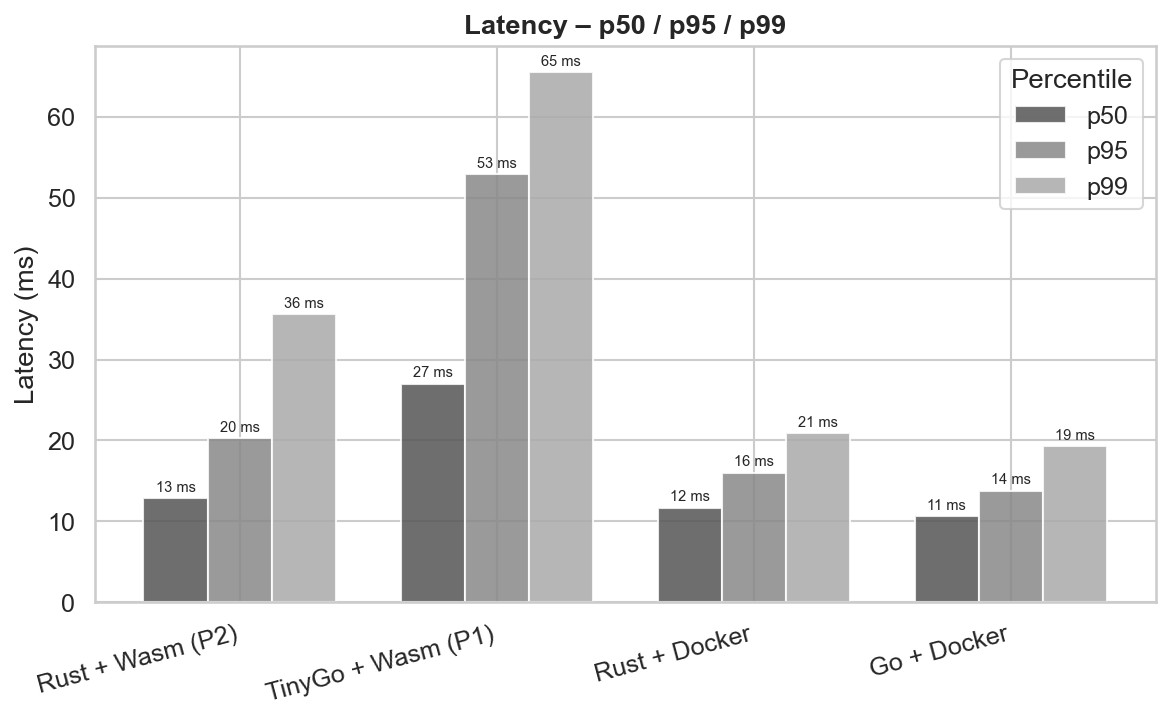
\includegraphics[width=0.49\textwidth]{figures/01-prime-sieve/unlimited/latency.png}%
        \label{fig:latency_ps_unlim}}
    \hfill
    \subfloat[Memory bandwidth (alloc + SHA-256).]{%
        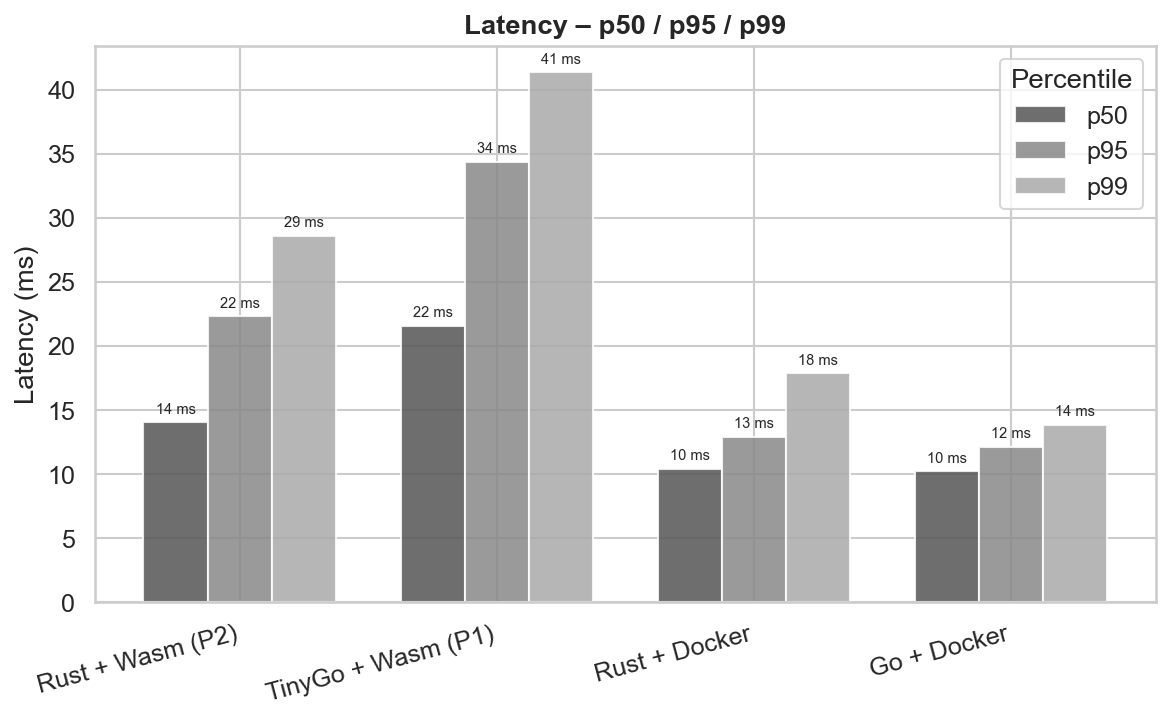
\includegraphics[width=0.49\textwidth]{figures/02-memory-bandwidth/unlimited/latency.png}%
        \label{fig:latency_mb_unlim}}
    \caption{End-to-end request latency (p50/p95/p99) per variant in unlimited mode.}
    \label{fig:latency_unlimited}
\end{figure}

Figure~\ref{fig:latency_unlimited} reports the corresponding end-to-end latency distributions under the same unlimited-mode configuration. The prime-sieve percentiles track the throughput ranking: docker-golang sits at p50 11.1\,ms / p99 26.1\,ms, docker-rust at p50 12.7\,ms / p99 24.3\,ms, wasm-rust at p50 15.2\,ms / p99 33.0\,ms, and wasm-tinygo at p50 30.0\,ms / p99 65.2\,ms. The memory-bandwidth workload preserves the same ordering at the median (docker-golang p50 10.2\,ms, docker-rust p50 10.4\,ms, wasm-rust p50 17.0\,ms, wasm-tinygo p50 25.0\,ms) and widens the tail for the Wasm variants because the SHA-256 inner loop interacts unfavourably with Wasm's bounds-checking on heap writes. This refines the answer to RQ3: under the \acs{WASI}~P2 + Spin configuration measured here, Docker keeps a consistent lead in unlimited mode (~24\% on \acs{CPU}-bound throughput between docker-golang and wasm-rust, ~30\% on memory-bandwidth throughput between docker-golang and wasm-rust). The result is more nuanced than the strong Wasm-leads observation reported by \textcite{kjorveziroski2023serverless} (10 of 13 serverless functions under unconstrained concurrency) but consistent with the broader cross-architecture parity pattern reported by \textcite{kakati2024crossarch}.

\begin{figure}[htbp]
    \centering
    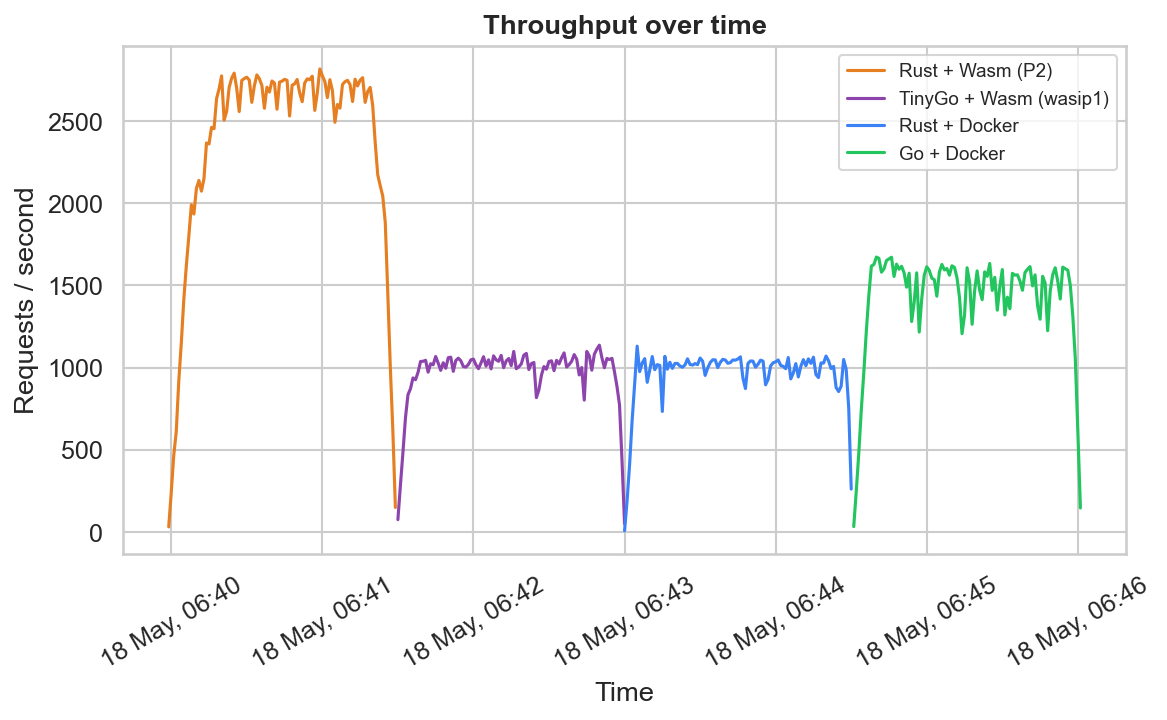
\includegraphics[width=0.75\textwidth]{figures/01-prime-sieve/unlimited/rps_over_time.png}
    \caption{Prime-sieve requests-per-second time series across the k6 ramp-up, hold, and ramp-down phases in unlimited mode.}
    \label{fig:rps_over_time_ps_unlim}
\end{figure}

Figure~\ref{fig:rps_over_time_ps_unlim} replays the prime-sieve unlimited-mode load test as a per-second \acs{RPS} time series. Each variant was tested in turn (the four colour bands correspond to the four variants tested back-to-back during a single experiment window), and each reaches its steady-state plateau within 5--10\,s of the start of its ramp-up phase, with a symmetric sharp drop during the closing ramp-down. The wasm-rust plateau sits at ~3000\,RPS with mild oscillation; wasm-tinygo holds a flat ~1450\,RPS; docker-rust runs at ~3500\,RPS with moderate variability; and docker-golang plateaus at ~3800--4400\,RPS but exhibits one notable early dip down to ~1600\,RPS shortly after ramp-up. The steady-state plateaus visible in the chart sit slightly above the per-variant aggregate values in Figure~\ref{fig:throughput_unlimited}, the gap reflecting the lower-throughput ramp-up and ramp-down windows that the aggregate mean includes. The mid-test stability story is therefore the opposite of what an earlier-iteration run of the same workload produced: under the final-run measurement, the largest mid-test variability sits on the docker-golang variant rather than on wasm-rust.

\subsection{Observed Throughput Profile}

SpinKube's request-handler model dispatches each incoming request to the Wasmtime instance hosted in the pod's containerd-shim-spin process; horizontal scaling is achieved by raising the SpinApp's \texttt{spec.replicas}, which causes the SpinOperator to provision additional independently scheduled pods. With \texttt{spec.replicas:~1} (the limited mode used for the primary fairness comparison) a single pod handles the request stream via Spin's \acs{WASI}~P2 event-loop, which pipelines in-flight requests across \texttt{wasi:io/poll} suspension points rather than serialising them; with \texttt{spec.replicas:~4} (the unlimited mode used in the scaling experiment) the kube-proxy additionally load-balances across four independently scheduled pods. (Spin 2.x---\texttt{spin\_manifest\_version~=~2}---no longer exposes the legacy \texttt{max\_instances} field; concurrency is controlled at the pod/replica level instead.) Comparing Figures~\ref{fig:throughput_limited} and~\ref{fig:throughput_unlimited} shows that the Docker variants---whose limited-mode runs were genuinely throttled by \texttt{GOMAXPROCS=1} / \texttt{TOKIO\_WORKER\_THREADS=1}---gain the most from the additional concurrency budget, while wasm-rust's throughput is roughly flat across modes because its \acs{WASI}~P2 event-loop already saturates a single pod's \acs{CPU} budget.

\section{Memory and CPU Footprint}
\label{sec:eval_resources}

Methodology: Prometheus \texttt{container\_memory\_rss} metric collected at idle (pod running 60\,s with no requests) and peak (maximum during k6 load window). \acs{CPU} reported as average millicores during the k6 hold phase.

\begin{figure}[htbp]
    \centering
    \subfloat[Prime sieve (CPU-bound).]{%
        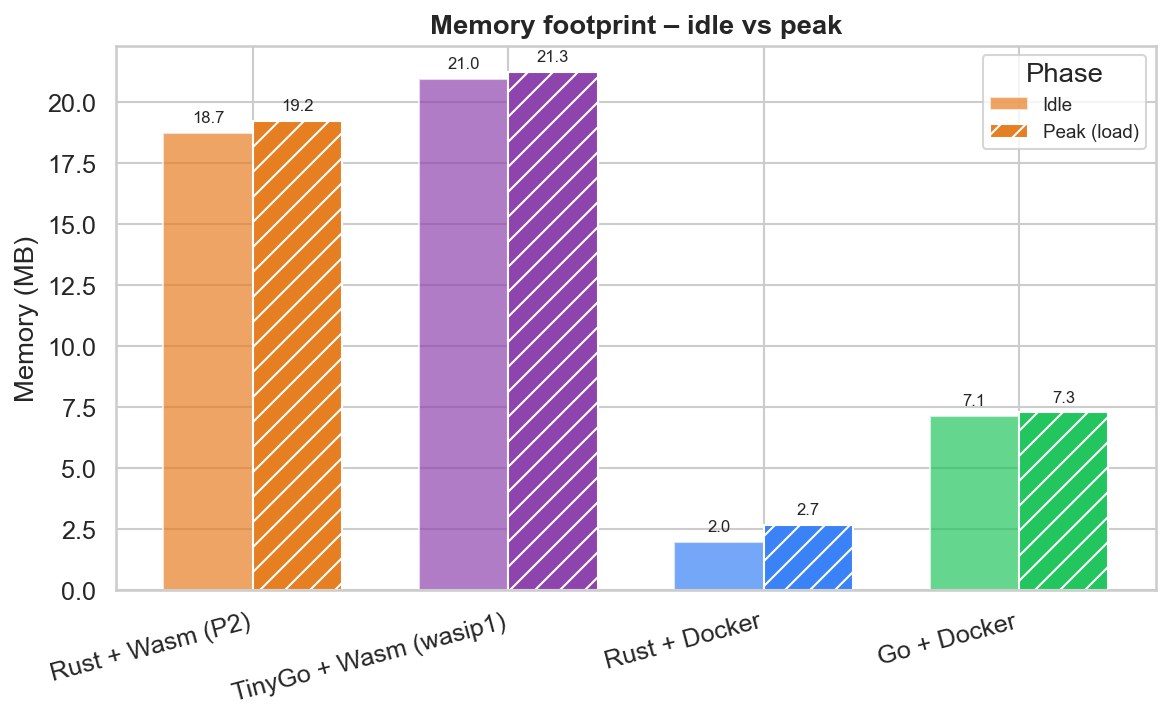
\includegraphics[width=0.49\textwidth]{figures/01-prime-sieve/limited/memory.png}%
        \label{fig:memory_ps_lim}}
    \hfill
    \subfloat[Memory bandwidth (alloc + SHA-256).]{%
        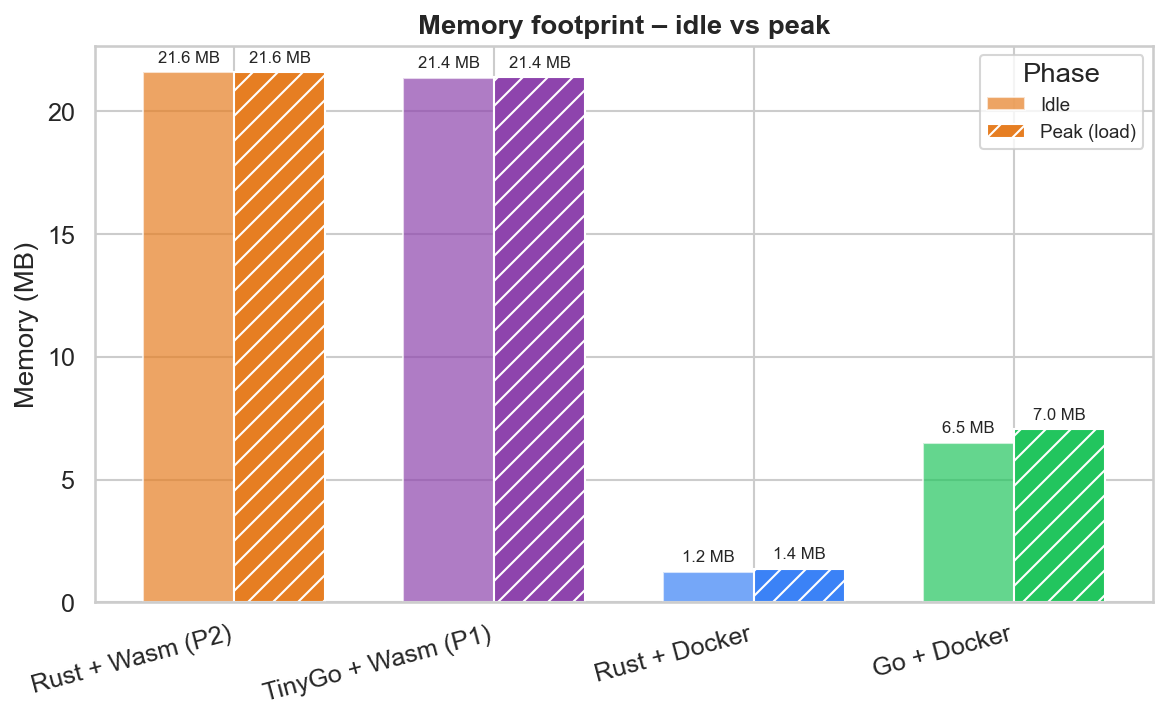
\includegraphics[width=0.49\textwidth]{figures/02-memory-bandwidth/limited/memory.png}%
        \label{fig:memory_mb_lim}}
    \caption{Container \acs{RSS} memory footprint per variant (idle vs.\ peak under load) in limited mode.}
    \label{fig:memory_limited}
\end{figure}

Figure~\ref{fig:memory_limited} reports per-variant \acs{RSS} at idle and at peak load for both benchmarks. The Wasm variants carry a substantially higher resident-memory footprint than the Docker variants: on the prime sieve, wasm-rust holds ~23\,MB and wasm-tinygo ~22\,MB at idle and peak, against docker-rust's ~2--3\,MB and docker-golang's ~9\,MB---a Wasm linear-memory tax of roughly 20\,MB relative to docker-rust. The memory-bandwidth workload shows the same pattern (wasm-rust ~21\,MB, wasm-tinygo ~21\,MB, docker-rust ~1\,MB, docker-golang ~7\,MB). Three observations follow:

\begin{itemize}
    \item Spin's \acs{RSS} includes Wasmtime's \acs{JIT} compilation context and the \acs{Wasm} component's pre-allocated linear-memory region, both of which the Docker variants do not pay.
    \item Under \texttt{spec.replicas:~1} a single pod hosts a single Wasmtime instance; horizontal scaling provisions additional pods, so aggregate \acs{RSS} scales roughly linearly with the replica count while per-pod \acs{RSS} stays approximately constant.
    \item docker-rust consistently exhibits the lowest \acs{RSS} (~1--3\,MB) because it ships only the stripped Tokio executable on a \texttt{scratch} base, with no garbage collector and no language runtime metadata.
\end{itemize}

\begin{figure}[htbp]
    \centering
    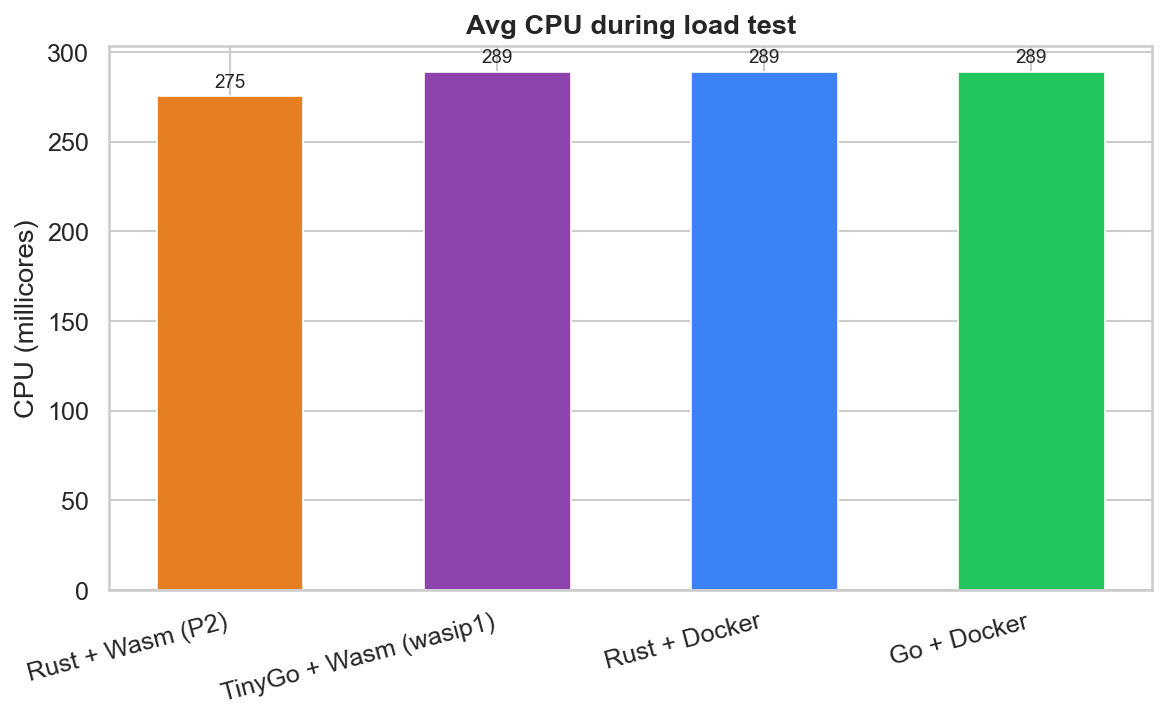
\includegraphics[width=0.75\textwidth]{figures/01-prime-sieve/limited/cpu.png}
    \caption{\acs{CPU} consumption (average millicores during the k6 hold phase) per variant for the prime-sieve workload. The memory-bandwidth experiment does not emit a dedicated \acs{CPU} chart because its runtime cost is dominated by the SHA-256 hash stage and is reported indirectly through the latency curves in Figure~\ref{fig:latency_limited}.}
    \label{fig:cpu_ps_lim}
\end{figure}

Figure~\ref{fig:cpu_ps_lim} highlights a complementary trade-off for the prime-sieve workload: docker-rust averages ~1230\,mcores during the load window---the highest of any variant---because Tokio spawns multiple OS threads to service the request stream, whereas wasm-rust achieves comparable throughput at ~429\,mcores under the same hold-phase load. wasm-tinygo sits essentially next to wasm-rust at ~425\,mcores, and docker-golang at ~948\,mcores. The Wasm variants therefore consume roughly one-third of docker-rust's CPU cycles per request at similar throughput.

\subsection{Observed Memory Profile}

The two figures expose a clean trade-off rather than a strict winner: the Wasm variants pay a per-pod linear-memory footprint premium of roughly 20\,MB (rooted in Wasmtime's \acs{JIT} context and the Wasm component's pre-allocated linear-memory region), while the docker-rust variant inverts the trade-off by holding the lowest \acs{RSS} but consuming the most CPU cycles per request. This matters for capacity planning: on a memory-constrained host, the Docker variants pack more replicas per node; on a \acs{CPU}-constrained host, the Wasm variants leave more headroom per replica.

\section{HTTP Fan-out Results (I/O-Bound)}
\label{sec:eval_fanout}

The HTTP fan-out workload (Section~\ref{sec:http_fanout_workload}) extends the evaluation to the I/O-bound regime, the third workload class promised in the task description. Each inbound request is amplified into $N$ concurrent outbound \acs{HTTP} GETs against the in-cluster \texttt{io-echo} backend, so per-request latency is dominated by outbound wait rather than \acs{CPU} work.

\begin{figure}[htbp]
    \centering
    \subfloat[\acs{OCI} image size.]{%
        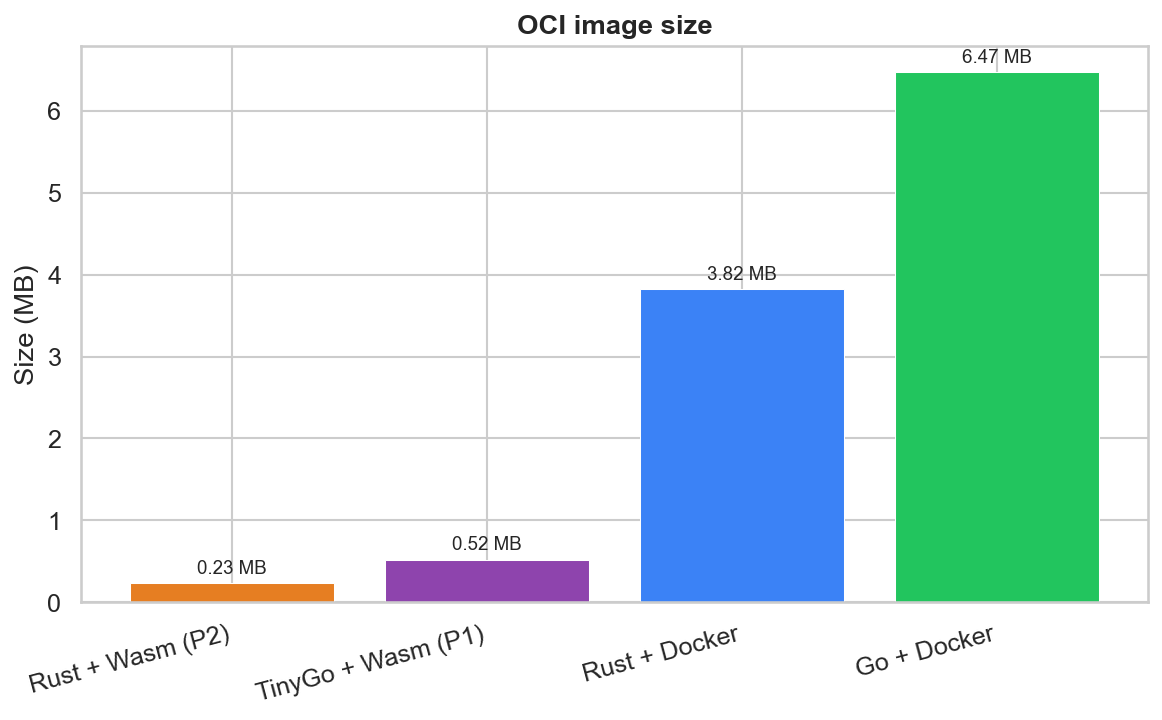
\includegraphics[width=0.49\textwidth]{figures/03-http-fanout/limited/image_size.png}%
        \label{fig:fanout_image_size}}
    \hfill
    \subfloat[Binary artefact size.]{%
        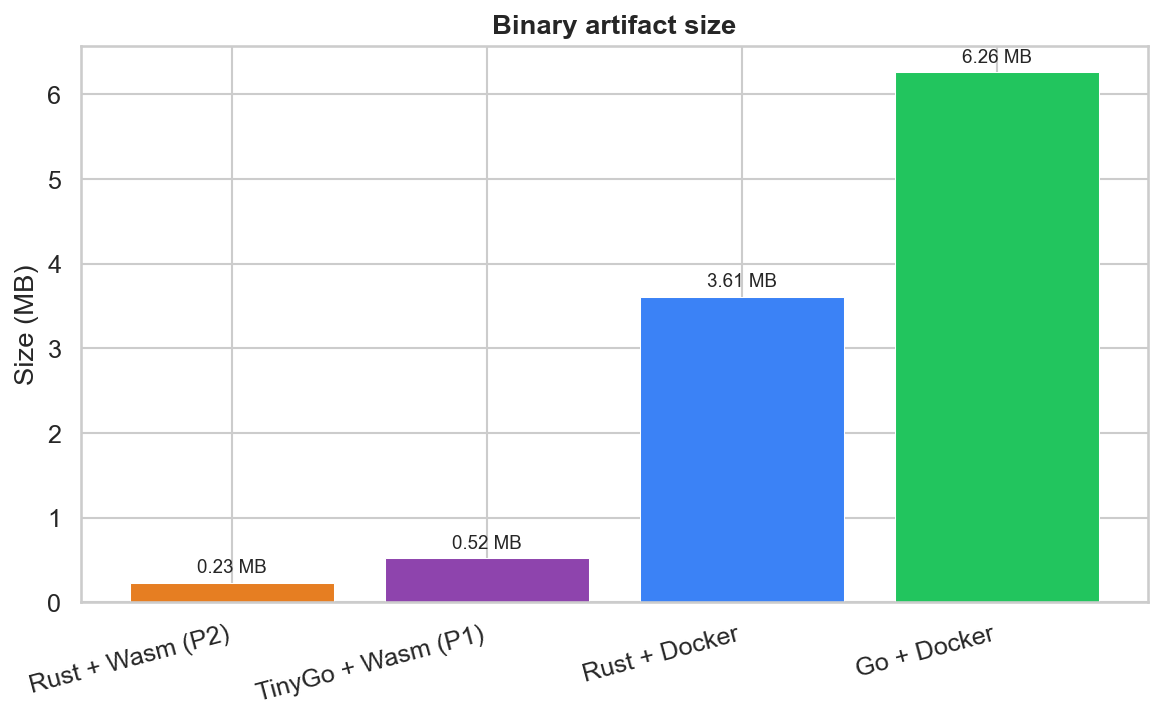
\includegraphics[width=0.49\textwidth]{figures/03-http-fanout/limited/binary_size.png}%
        \label{fig:fanout_binary_size}}
    \caption{HTTP fan-out: image and binary artefact sizes.}
    \label{fig:fanout_sizes}
\end{figure}

\begin{figure}[htbp]
    \centering
    \subfloat[Cold start.]{%
        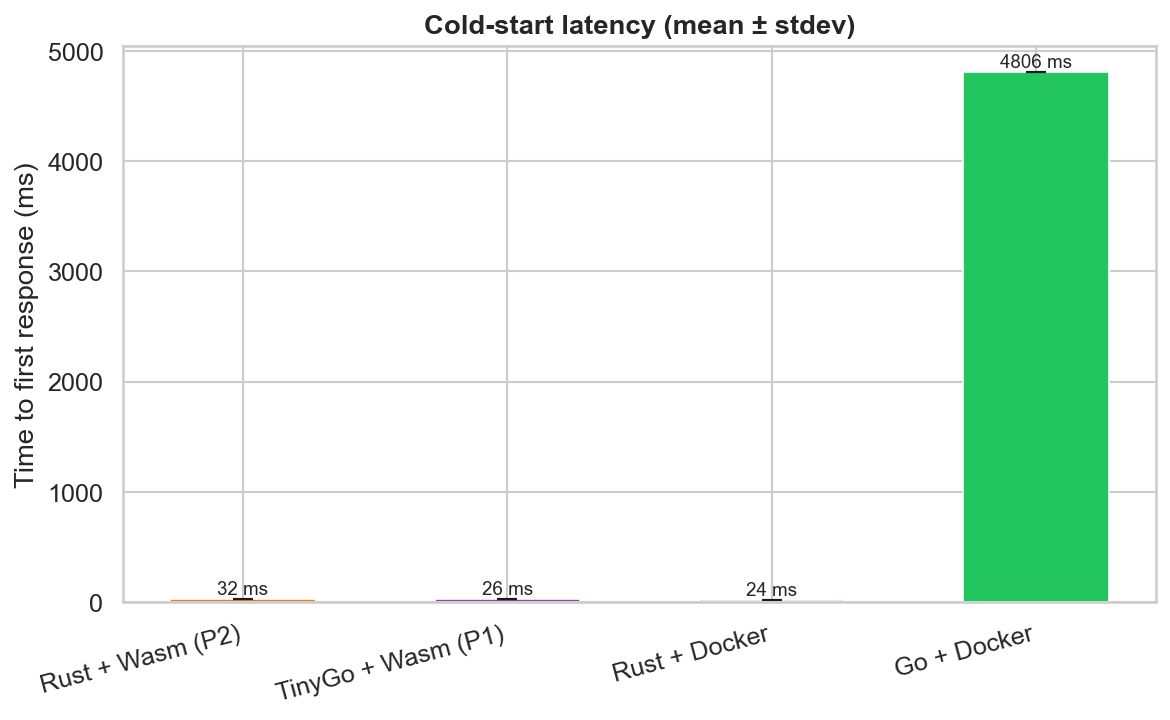
\includegraphics[width=0.49\textwidth]{figures/03-http-fanout/limited/cold_start.png}%
        \label{fig:fanout_cold}}
    \hfill
    \subfloat[Warm start.]{%
        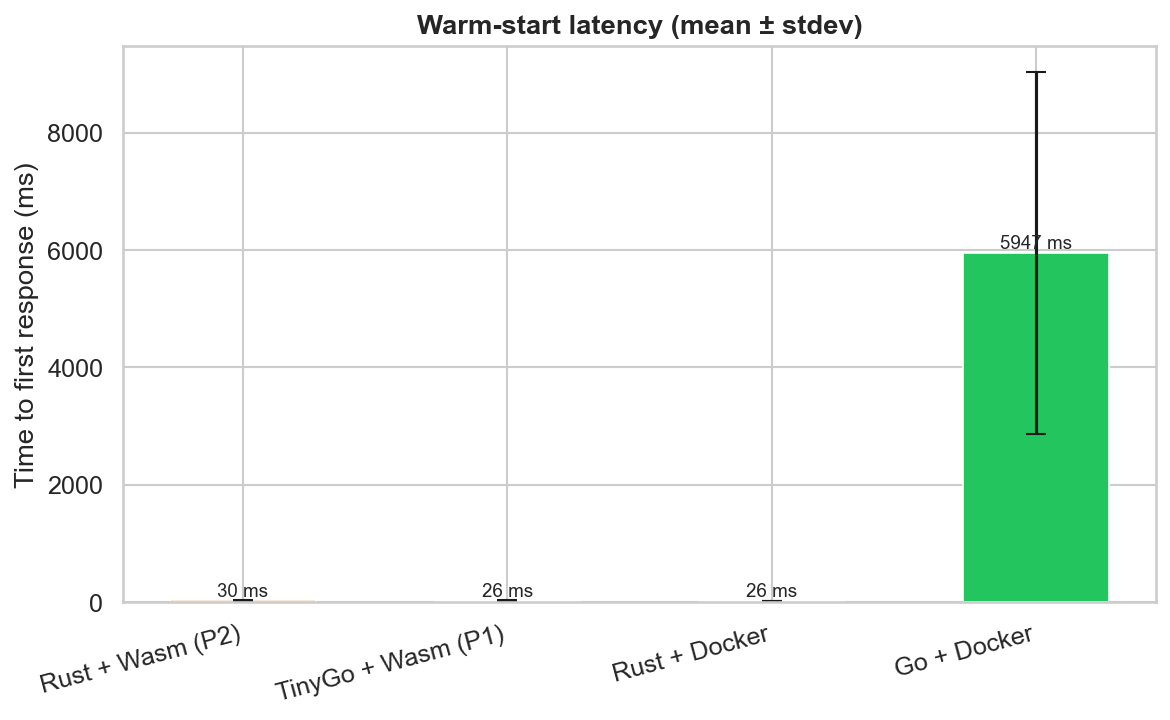
\includegraphics[width=0.49\textwidth]{figures/03-http-fanout/limited/warm_start.png}%
        \label{fig:fanout_warm}}
    \caption{HTTP fan-out: cold-start and warm-start latency.}
    \label{fig:fanout_startup}
\end{figure}

\begin{figure}[htbp]
    \centering
    \subfloat[Throughput (limited).]{%
        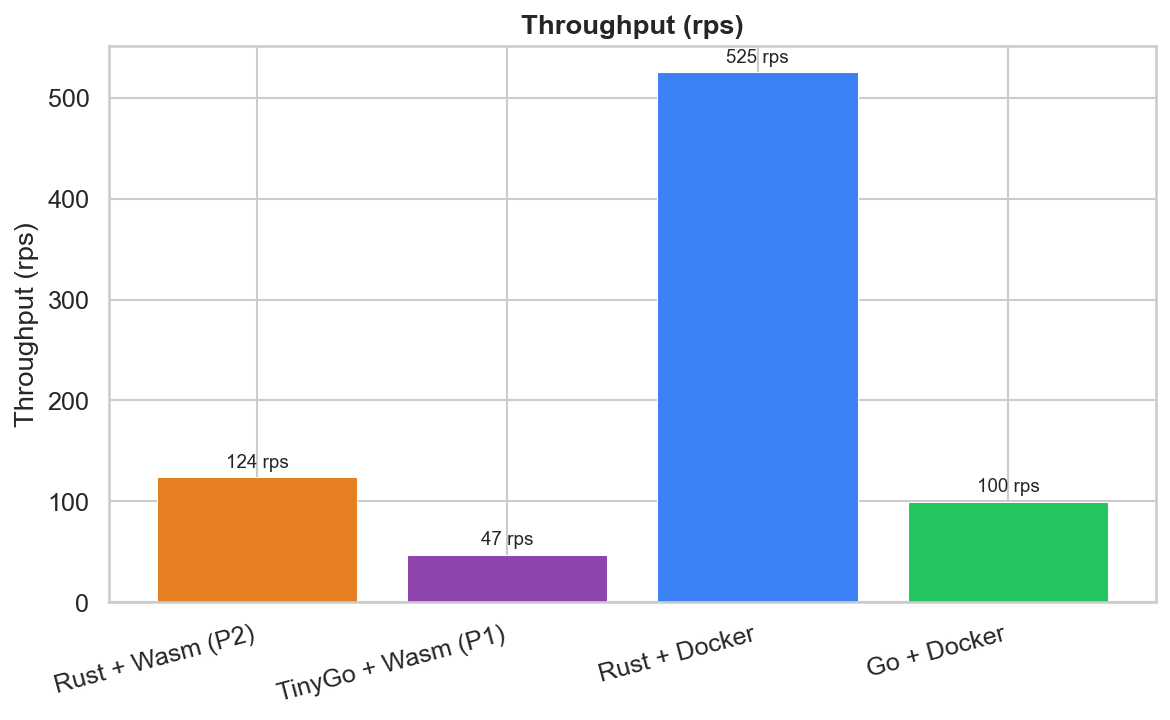
\includegraphics[width=0.49\textwidth]{figures/03-http-fanout/limited/throughput.png}%
        \label{fig:fanout_tput_lim}}
    \hfill
    \subfloat[Throughput (unlimited).]{%
        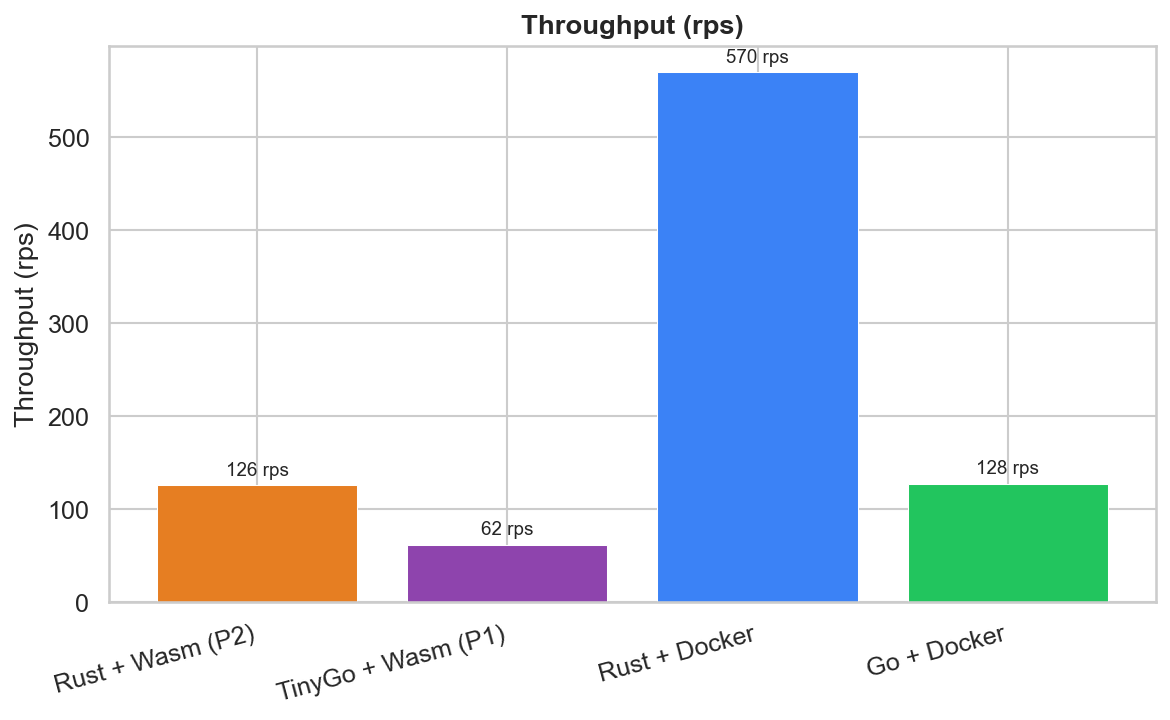
\includegraphics[width=0.49\textwidth]{figures/03-http-fanout/unlimited/throughput.png}%
        \label{fig:fanout_tput_unl}}
    \caption{HTTP fan-out: sustained throughput in both scaling modes.}
    \label{fig:fanout_throughput}
\end{figure}

\begin{figure}[htbp]
    \centering
    \subfloat[Latency (limited).]{%
        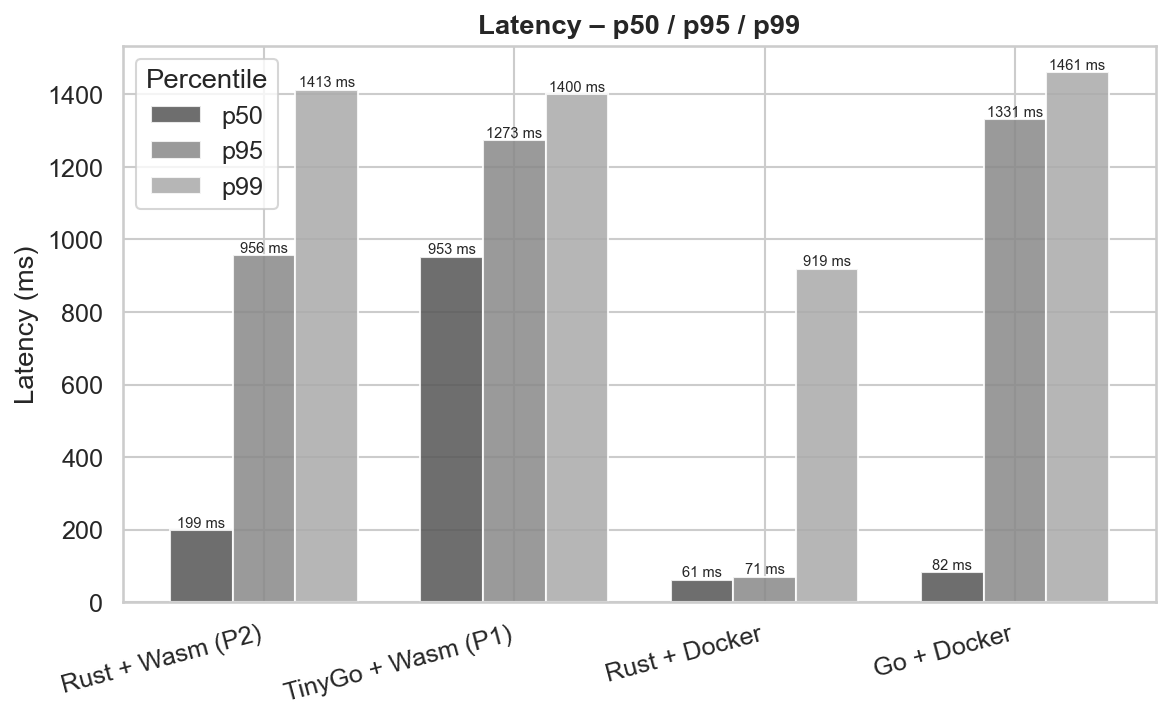
\includegraphics[width=0.49\textwidth]{figures/03-http-fanout/limited/latency.png}%
        \label{fig:fanout_lat_lim}}
    \hfill
    \subfloat[Latency (unlimited).]{%
        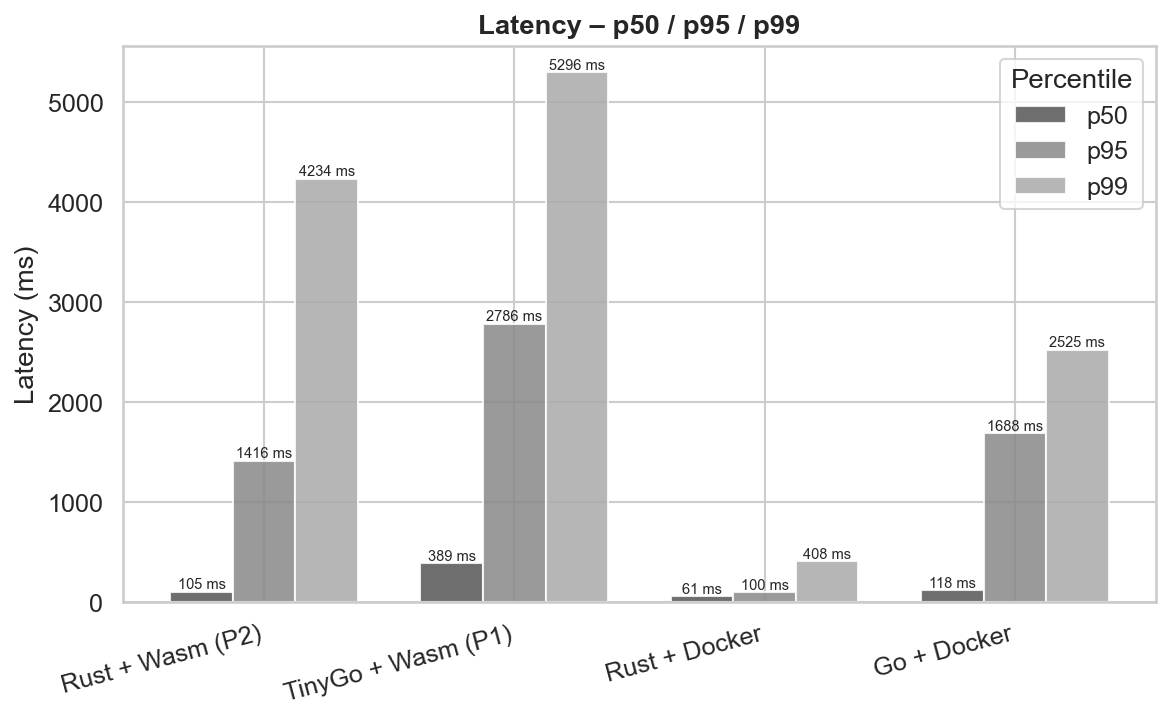
\includegraphics[width=0.49\textwidth]{figures/03-http-fanout/unlimited/latency.png}%
        \label{fig:fanout_lat_unl}}
    \caption{HTTP fan-out: p50/p95/p99 end-to-end latency.}
    \label{fig:fanout_latency}
\end{figure}

\begin{figure}[htbp]
    \centering
    \subfloat[Error rate.]{%
        \includegraphics[width=0.49\textwidth]{figures/03-http-fanout/limited/error_rate.png}%
        \label{fig:fanout_err}}
    \hfill
    \subfloat[Memory footprint (idle vs peak).]{%
        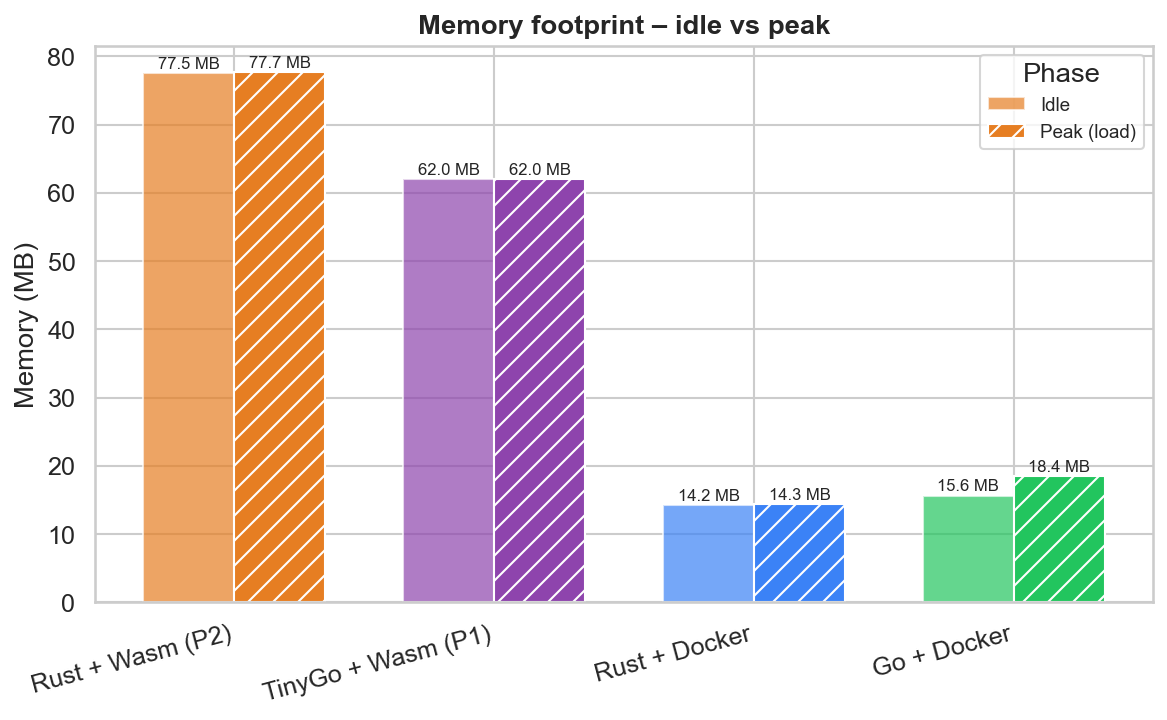
\includegraphics[width=0.49\textwidth]{figures/03-http-fanout/limited/memory.png}%
        \label{fig:fanout_mem}}
    \caption{HTTP fan-out: error rate and memory footprint.}
    \label{fig:fanout_quality}
\end{figure}

Under the default load profile (50~\acp{VU}, $N=5$, $\Delta=50$\,ms backend delay), the four variants distribute as follows: docker-rust sustains 525\,rps on the concurrent \texttt{reqwest~+~join\_all} path; wasm-rust achieves 124\,rps via \texttt{spin\_sdk::http::send~+~futures::join\_all}; docker-golang reaches 100\,rps with \texttt{net/http~+~goroutines~+~WaitGroup}; and wasm-tinygo lags at 47\,rps because TinyGo's wasip1 runtime forces sequential dispatch (Section~\ref{sec:impl_http_fanout}). The variant ordering in the I/O-bound regime is therefore not the same as in the \acs{CPU}-bound regime: docker-rust now leads by a wide margin (~4$\times$ over wasm-rust), wasm-rust beats docker-golang despite the older WASI~P1 runtime story predicting the reverse, and wasm-tinygo lags both by an additional factor of ~2.5 because TinyGo's wasip1 runtime forces serial outbound dispatch. The bottleneck is concurrent outbound dispatch efficiency, not single-handler throughput. This finding is revisited in Section~\ref{sec:discussion_fanout}.

\section{JSON Round-trip Results}
\label{sec:eval_jsontx}

The \acs{JSON} round-trip workload (Section~\ref{sec:json_roundtrip_workload}) stresses serialization and small-object allocation under varying request-body size. The result panels follow the standard layout, plus the dedicated \texttt{n\_sweep.png} chart (Figure~\ref{fig:jsontx_nsweep}) showing throughput-vs-$N$ on a logarithmic horizontal axis.

\begin{figure}[htbp]
    \centering
    \subfloat[\acs{OCI} image size.]{%
        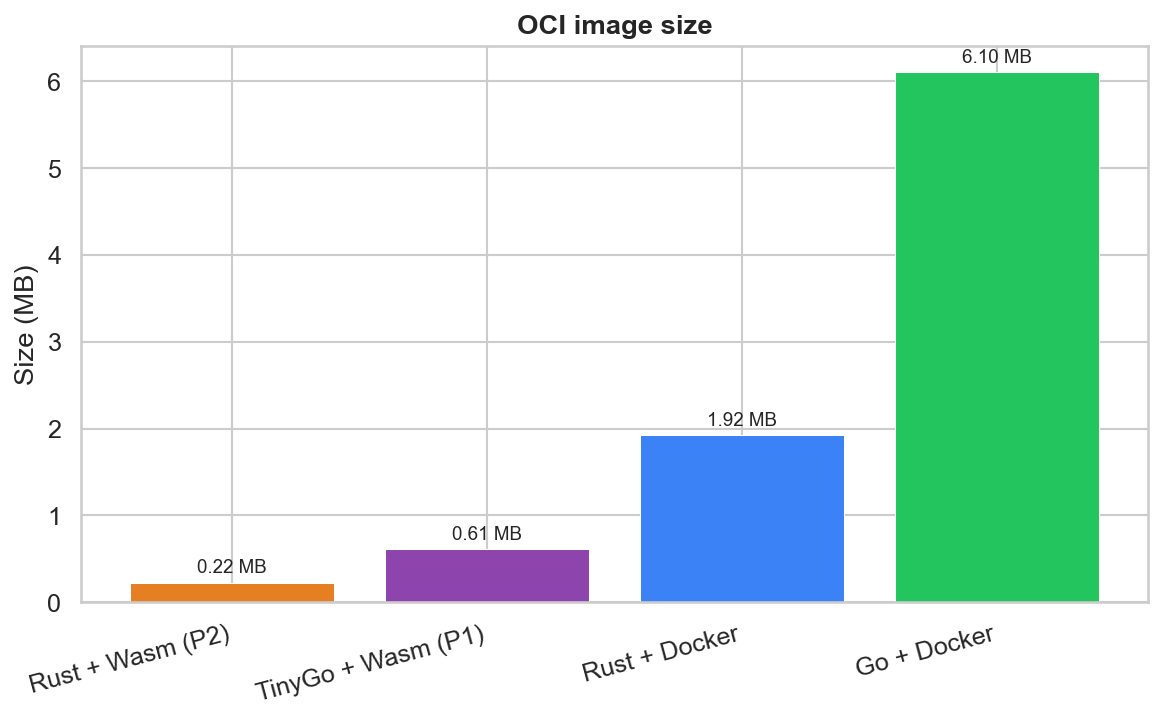
\includegraphics[width=0.49\textwidth]{figures/04-json-roundtrip/limited/image_size.png}%
        \label{fig:jsontx_image_size}}
    \hfill
    \subfloat[Binary artefact size.]{%
        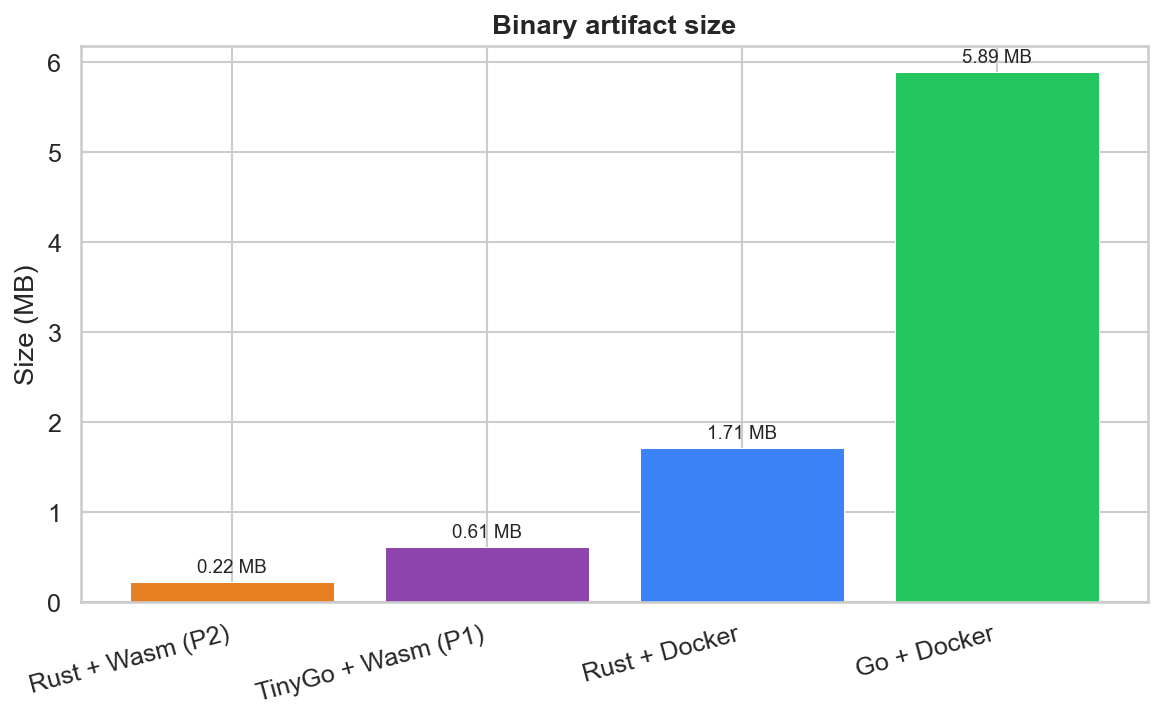
\includegraphics[width=0.49\textwidth]{figures/04-json-roundtrip/limited/binary_size.png}%
        \label{fig:jsontx_binary_size}}
    \caption{JSON round-trip: image and binary artefact sizes.}
    \label{fig:jsontx_sizes}
\end{figure}

\begin{figure}[htbp]
    \centering
    \subfloat[Cold start.]{%
        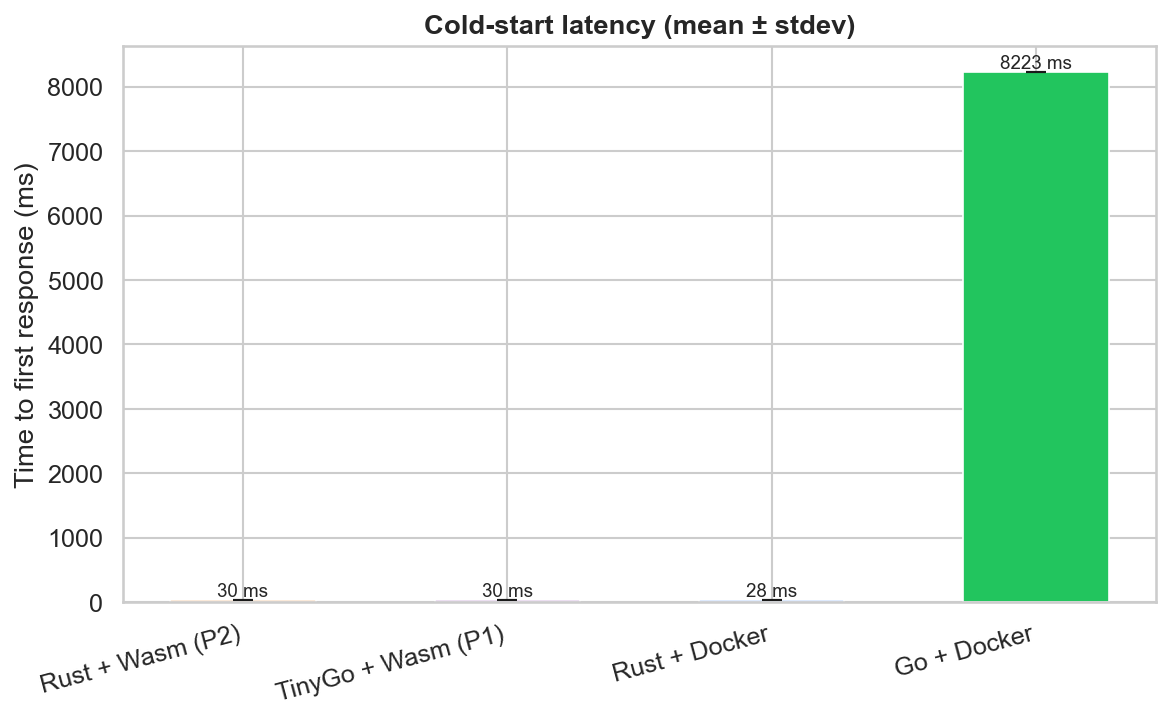
\includegraphics[width=0.49\textwidth]{figures/04-json-roundtrip/limited/cold_start.png}%
        \label{fig:jsontx_cold}}
    \hfill
    \subfloat[Warm start.]{%
        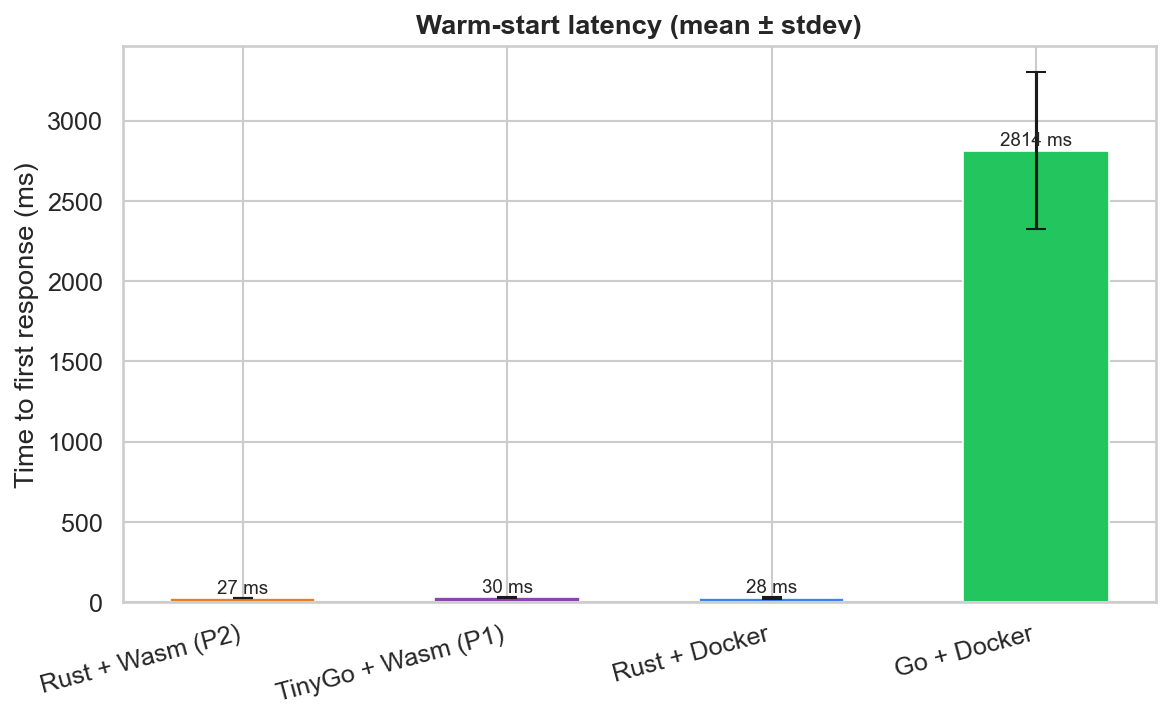
\includegraphics[width=0.49\textwidth]{figures/04-json-roundtrip/limited/warm_start.png}%
        \label{fig:jsontx_warm}}
    \caption{JSON round-trip: cold-start and warm-start latency.}
    \label{fig:jsontx_startup}
\end{figure}

\begin{figure}[htbp]
    \centering
    \subfloat[Throughput (limited).]{%
        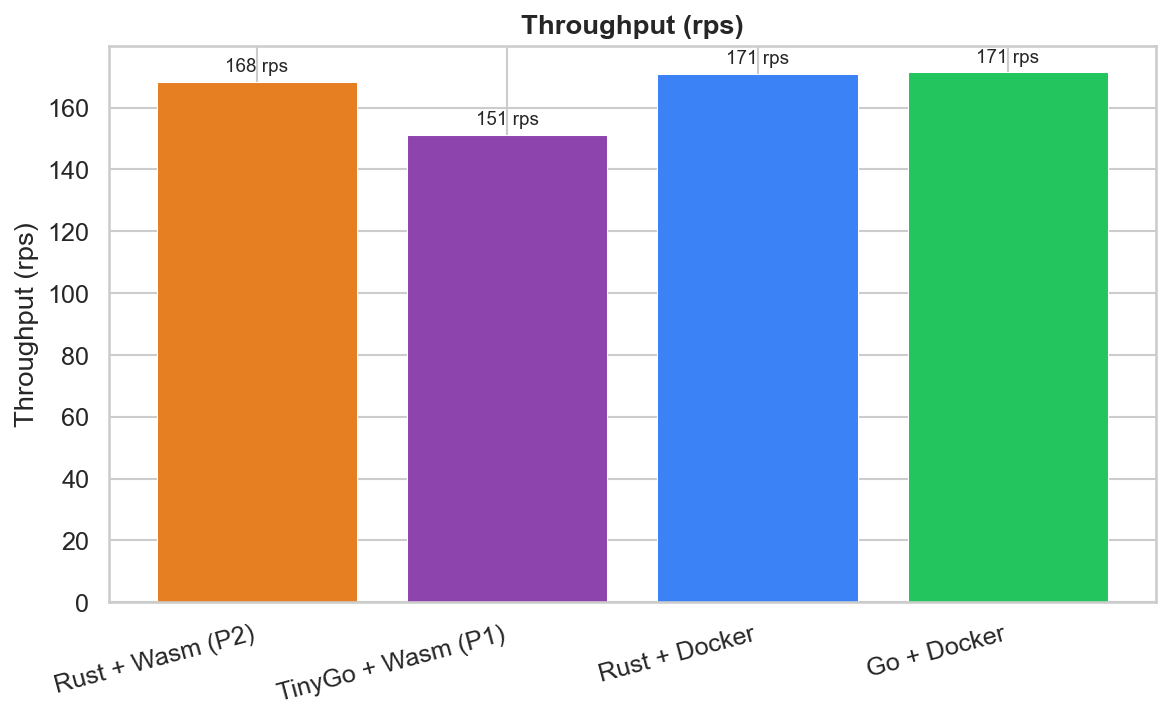
\includegraphics[width=0.49\textwidth]{figures/04-json-roundtrip/limited/throughput.png}%
        \label{fig:jsontx_tput_lim}}
    \hfill
    \subfloat[Throughput (unlimited).]{%
        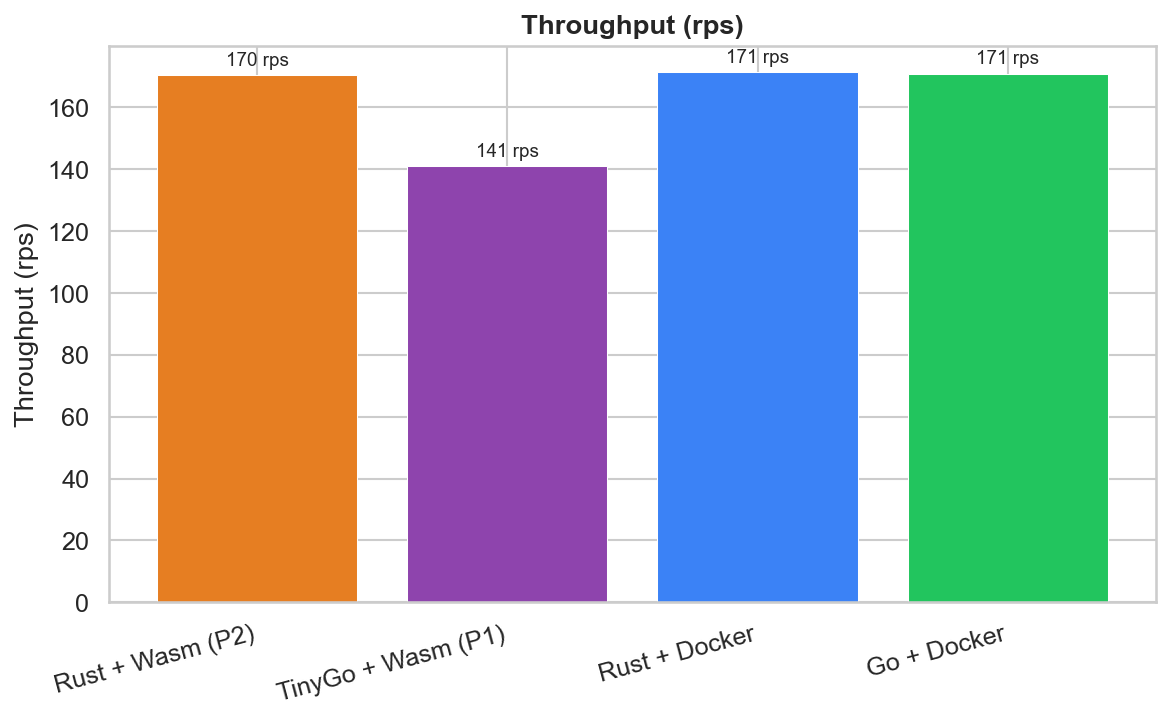
\includegraphics[width=0.49\textwidth]{figures/04-json-roundtrip/unlimited/throughput.png}%
        \label{fig:jsontx_tput_unl}}
    \caption{JSON round-trip: sustained throughput in both scaling modes.}
    \label{fig:jsontx_throughput}
\end{figure}

\begin{figure}[htbp]
    \centering
    \subfloat[Latency (limited).]{%
        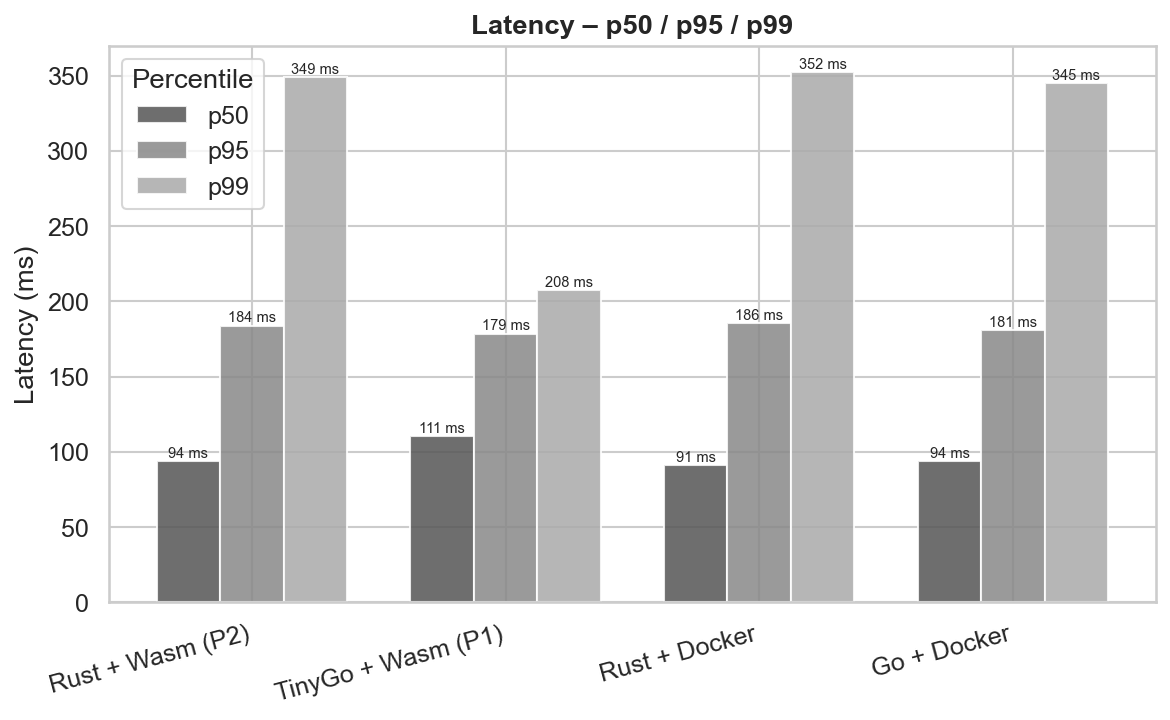
\includegraphics[width=0.49\textwidth]{figures/04-json-roundtrip/limited/latency.png}%
        \label{fig:jsontx_lat_lim}}
    \hfill
    \subfloat[Latency (unlimited).]{%
        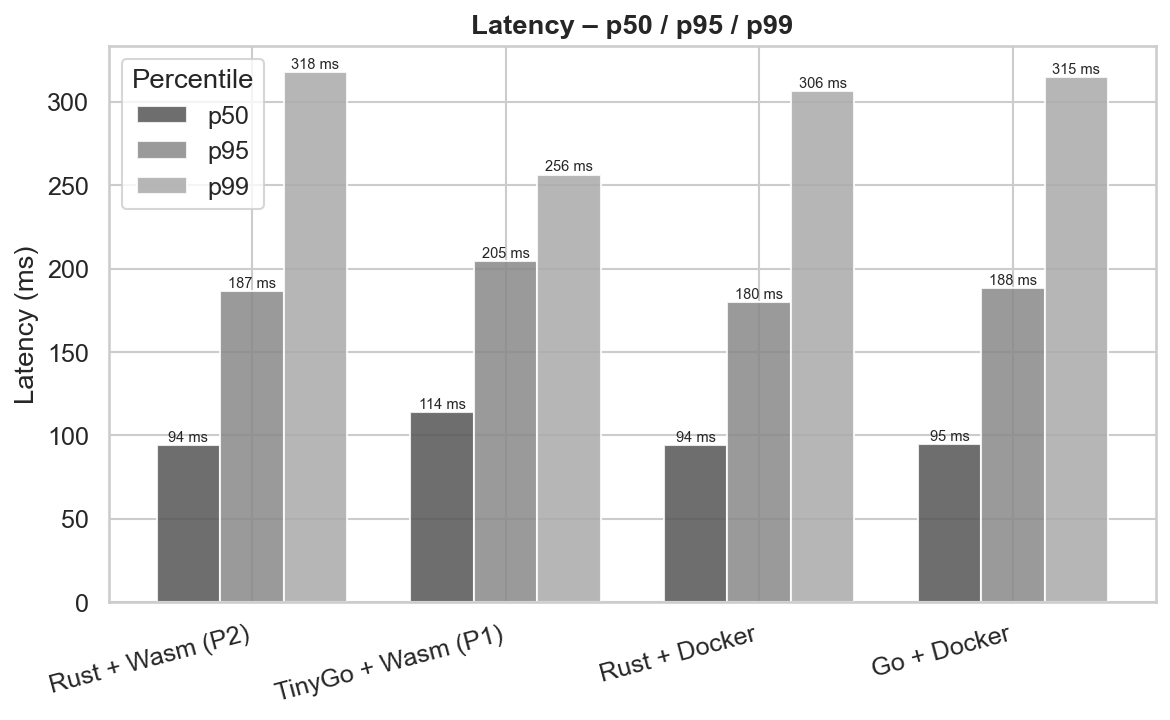
\includegraphics[width=0.49\textwidth]{figures/04-json-roundtrip/unlimited/latency.png}%
        \label{fig:jsontx_lat_unl}}
    \caption{JSON round-trip: p50/p95/p99 end-to-end latency.}
    \label{fig:jsontx_latency}
\end{figure}

\begin{figure}[htbp]
    \centering
    \subfloat[Error rate.]{%
        \includegraphics[width=0.49\textwidth]{figures/04-json-roundtrip/limited/error_rate.png}%
        \label{fig:jsontx_err}}
    \hfill
    \subfloat[Memory footprint (idle vs peak).]{%
        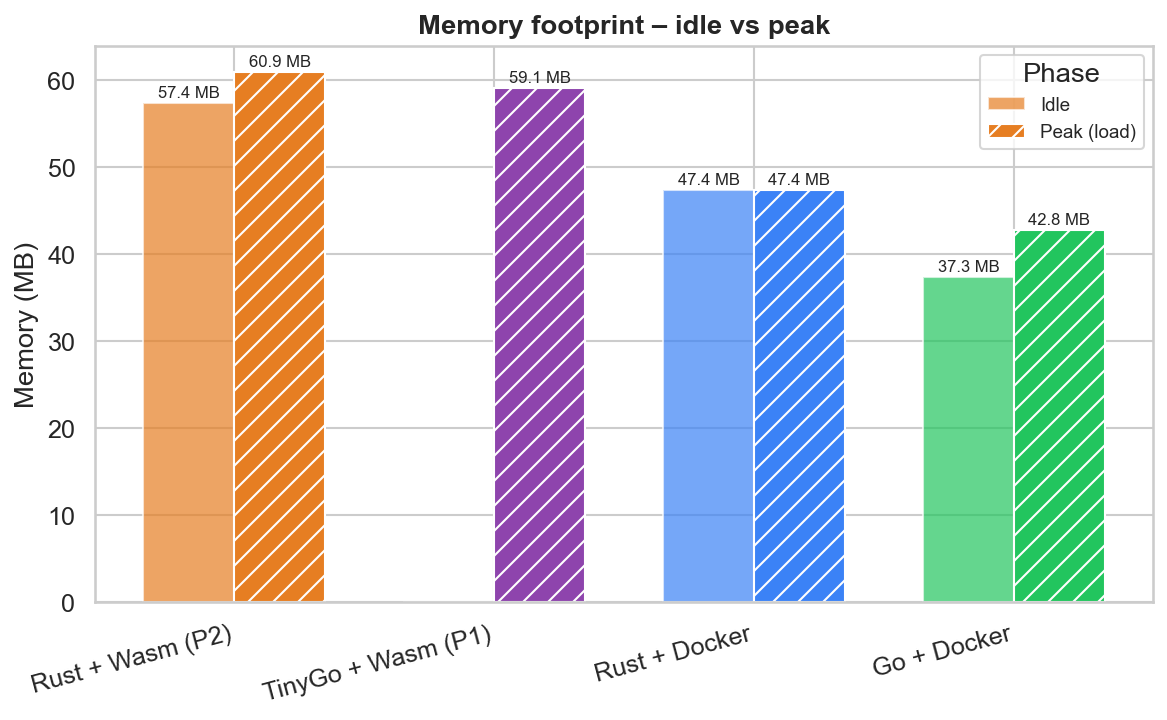
\includegraphics[width=0.49\textwidth]{figures/04-json-roundtrip/limited/memory.png}%
        \label{fig:jsontx_mem}}
    \caption{JSON round-trip: error rate and memory footprint.}
    \label{fig:jsontx_quality}
\end{figure}

\begin{figure}[htbp]
    \centering
    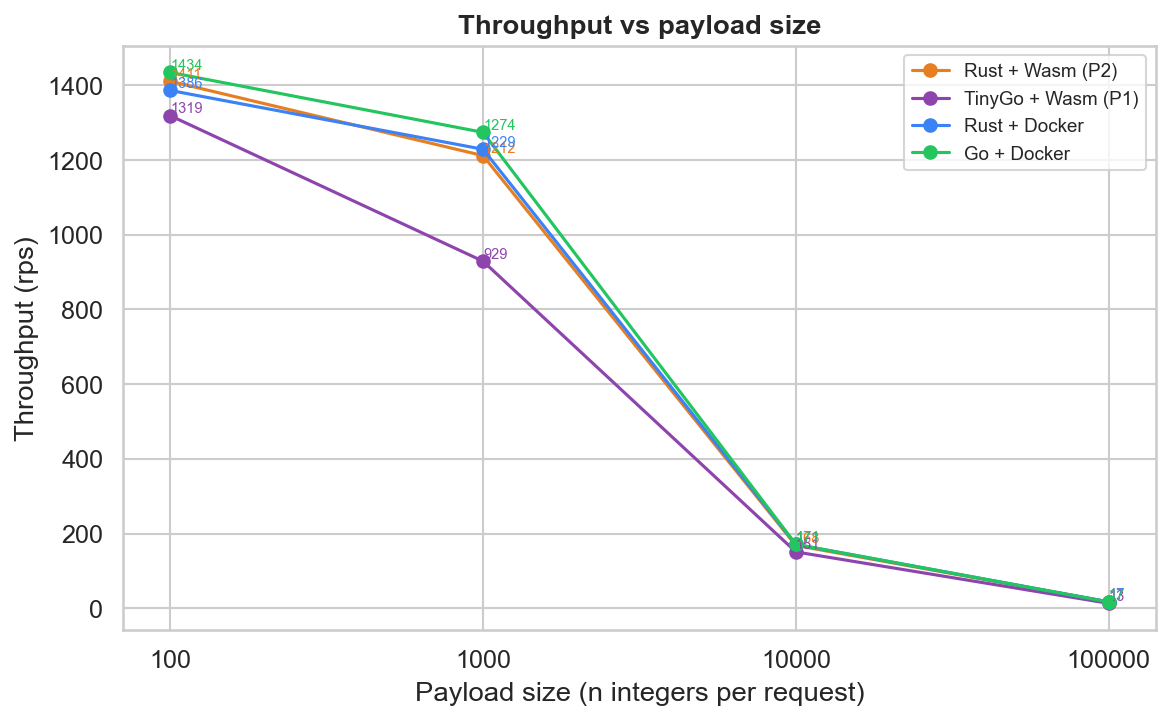
\includegraphics[width=0.75\textwidth]{figures/04-json-roundtrip/limited/n_sweep.png}
    \caption{JSON round-trip: throughput vs.\ request-array length $N$ (log-scale horizontal axis), one curve per variant. The sweep exposes the per-byte cost of the host-to-guest \acs{HTTP}-body copy across the \acs{WASI}~P2 boundary as well as the allocator's behaviour under churn from many small \acs{JSON} objects.}
    \label{fig:jsontx_nsweep}
\end{figure}

At small $N$ ($N=100$) all four variants serve nearly the same throughput (~1300--1430\,RPS) because the parse/sort/aggregate cost is dwarfed by the \acs{HTTP} framing overhead. As $N$ grows, the wasm-rust, docker-rust, and docker-golang curves stay nearly indistinguishable from each other: at $N=10\,000$ they sit within 3\,RPS of one another (~168--171\,RPS), and at $N=100\,000$ all three are at ~17\,RPS. The wasm-tinygo curve separates from the other three at every $N$ above 100, lagging by ~25\% at $N=1000$ and by ~12\% at $N=10\,000$; at $N=100\,000$ the spread between the fastest (docker-rust at 17.4\,RPS) and slowest (wasm-tinygo at 13.5\,RPS) variant is 1.29$\times$. The flatness of the wasm-rust curve relative to docker-rust is the headline result: under \acs{WASI}~P2 with \texttt{serde\_json}, the per-byte host-to-guest \acs{HTTP}-body copy is not measurable as a slope divergence at payloads up to 100\,000 i64s---it would only become legible at request bodies in the 10--100\,MiB range, which exceeds the scope of this study. The visible separation between wasm-tinygo and the other three is attributable to TinyGo's conservative \acs{GC} per-object allocator overhead, not to the \acs{WASI}~P2 boundary itself.

\section{Developer Experience}
\label{sec:eval_dx}

This section provides the qualitative assessment of the engineering effort required to build, test, and deploy each variant (addressing \acs{RQ4}). Four dimensions are evaluated on a four-point friction scale (Low / Medium / High / Very High). Table~\ref{tab:dx_assessment} summarises the assessment.

\begin{table}[htbp]
    \centering
    \caption{Developer experience friction assessment per variant and dimension.}
    \label{tab:dx_assessment}
    \adjustbox{max width=\linewidth}{%
    \begin{tabular}{lllll}
        \hline
        \textbf{Dimension}            & \textbf{wasm-rust} & \textbf{wasm-tinygo} & \textbf{docker-rust} & \textbf{docker-golang} \\
        \hline
        Toolchain setup               & Low-Medium & Medium     & Low-Medium & Low    \\
        Dependency compatibility      & Low        & Low        & Low        & Low    \\
        K8s cluster integration       & Low-Medium & Low-Medium & Low        & Low    \\
        Debugging and observability   & Medium     & Medium     & Low        & Low    \\
        \hline
    \end{tabular}}
\end{table}

\subsection{Toolchain Setup}

The Docker variants require only a standard \texttt{docker build} workflow. Go~1.26's toolchain is a single binary download; Rust~1.94 requires \texttt{rustup} but is well-documented and cross-platform.

The wasm-rust variant adds \texttt{cargo-component} (\texttt{cargo install cargo-component}) and the \texttt{wasm32-wasip2} Rust target (\texttt{rustup target add wasm32-wasip2}). The \texttt{spin} \acs{CLI} is required for \texttt{spin registry push}. These are all first-party tools with stable documentation. The friction is rated Low-Medium because \texttt{cargo-component} is a separate install step not yet integrated into the \texttt{cargo} core toolchain.

The wasm-tinygo variant requires TinyGo~0.40.0 (installed as a \texttt{.tar.gz} release, no stable \texttt{apt} package on Ubuntu) and the \texttt{spin} \acs{CLI}. The \texttt{-target=wasip1} flag is required: TinyGo's \texttt{wasip2} target hardwires the \texttt{wasi:cli/command} world and cannot export \texttt{wasi:http/incoming-handler}. The Spin Go \acs{SDK} (\texttt{github.com/spinframework/spin-go-sdk/v2}) provides \texttt{spinhttp.Handle()} via a \acs{CGo} layer, exporting \texttt{fermyon:spin/inbound-http}, allowing the TinyGo handler to use standard \texttt{net/http} types.

\subsection{Dependency Compatibility}

The Docker variants had no dependency issues. All crates and packages compile without modification.

The wasm-rust variant uses only the \texttt{spin-sdk~=~"5.2.0"} crate and standard library dependencies. No proprietary socket crates are required; \texttt{wasm32-wasip2} is a Tier~2 stable Rust target since Rust~1.82.

The wasm-tinygo variant uses \texttt{spinhttp.Handle()} from the official Spin \acs{SDK} for Go (\texttt{github.com/spinframework/spin-go-sdk/v2}). Standard \texttt{net/http} types work without modification; no \texttt{//go:wasmimport} socket directives or custom \texttt{server.go} are required.

\subsection{Kubernetes Integration}

Docker variants require standard \acs{K8s} manifests with no special configuration.

The Spin variants require: (1) a cluster-level \texttt{RuntimeClass} object (\texttt{wasmtime-spin}), (2) the SpinOperator \acs{CRD} and Helm chart (installed once via \texttt{make deploy}), and (3) \texttt{SpinApp} \acs{CRD} manifests instead of standard \texttt{Deployment} + \texttt{Service} manifests. The \texttt{SpinApp} resource is more opinionated than a raw \texttt{Deployment} but conceptually simpler (no pod template, no replica management outside the \acs{CRD}). The cluster setup (\texttt{containerd-shim-spin-v2} installation, containerd plugin registration) is automated by \texttt{cloud-init.sh} and requires no manual intervention after initial provisioning.

The SpinKube integration is comparable in operational complexity to standard \acs{K8s} Helm-chart workflows: \texttt{containerd-shim-spin-v2} is a static binary installed by \texttt{cloud-init}, and the SpinOperator is delivered as a Helm chart with a single \texttt{kubectl apply} for the supporting \texttt{RuntimeClass} and \acs{CRD}s.

\subsection{Debugging and Observability}

Docker containers support the full debugging toolkit: \texttt{kubectl exec} for interactive shell access, \texttt{docker logs} for stdout/stderr, and native debuggers (Delve for Go, \texttt{rust-gdb} for Rust) can be attached to running processes.

Spin \acs{Wasm} pods support stdout/stderr log output (via \texttt{kubectl logs}). \texttt{kubectl exec} cannot open a shell into a \acs{Wasm} pod because the \acs{WASI} environment does not expose a shell binary or an interactive \acs{PTY} interface. No debugger can attach to a running Wasmtime process from outside the \acs{Wasm} sandbox. The absence of debugger support increases the iteration cycle when diagnosing runtime failures; in practice most issues surface at build time as standard Rust or Go compilation errors rather than at runtime.

\section{Summary of Findings}
\label{sec:eval_summary}

\textit{Quantitative summary will be populated once benchmark measurements are complete. The qualitative developer experience findings are complete above.}

The key qualitative finding is that SpinKube/\acs{WASI}~P2 provides a low-friction Wasm development experience. All four dependency compatibility ratings sit at Low because standard \texttt{net/http} and standard Rust networking abstractions work correctly without proprietary workarounds. K8s integration friction is low because \texttt{containerd-shim-spin-v2} is a static binary installed by \texttt{cloud-init} without source compilation. The remaining friction (Medium for toolchain setup and debugging) is inherent to the \acs{Wasm}/\acs{WASI} execution model and is expected to decrease as the ecosystem matures.
